%{\let\clearpage\relax \chapter*{Содержание работы}}
%\section*{Содержание работы}
\chapter*{Содержание работы}
В диссертации проводится теоретическое изучение относительно нового метода формирования трехмерных микро-и наноструктур -- сухого электронно-лучевого травления резиста (СЭЛТР). 

В начале \underline{\textbf{первой главы}} приводится описание основных методов микро- и наноструктурирования, существующих в настоящее время -- наноимпринтной литографии~\cite{NIL_1}, двухфотонной лазерной литографии~\cite{TPL_castle}, интерференционной литографии~\cite{IL_metamaterials}, полутоновой литографии~\cite{GL_general} и сканирующей зондовой литографии~\cite{SPL_mechanical}. Исходя из их преимуществ и недостатков делается заключение о том, что в настоящее время отсутствует метод, обеспечивающий высокую производительность и являющийся в то же время простым в реализации.

Далее рассматривается концепция микролитографии на основе локальной термической деполимеризации резиста и описываются первые шаги в разработке метода сухого электронно-лучевого травления резиста. Описанные в работах~\cite{Bruk_2013, Bruk_2016_mee} эксперименты демонстрируют высокую производительность метода, а также сглаженный профиль получаемых структур (рис.~\ref{fig:DEBER_many_profiles}). При этом отмечается низкое латеральное разрешение метода, которое заметно ограничивает его область применимости. Поскольку при сухом электронно-лучевом травлении резиста профиль линии формируется под влиянием нескольких одновременно протекающих процессов, определение влияния каждого из них на результирующий профиль, разработка методов оптимизации метода СЭЛТР и оценка его возможностей на основе лишь экспериментальных исследований было затруднительным. И хотя основные процессы, протекающие при СЭЛТР (рассеяние электронного пучка в резисте и подложке, электронно-стимулированные разрывы молекул резиста, цепная деполимеризация резиста, диффузия мономера и растекание резиста) являются относительно хорошо изученными, их совместное протекание в процессе микроструктурирования до настоящего момента не исследовалось. Таким образом, целесообразным являлась разработка физической модели данного метода, верифицированной на основе имеющихся экспериментальных данных и позволяющей определить предельное разрешение метода, а также оценить возможность его применения для формирования необходимых структур.

\begin{figure}
	\centering
%	\includegraphics{jpg/DEBER_many_profiles_14pt_300}
	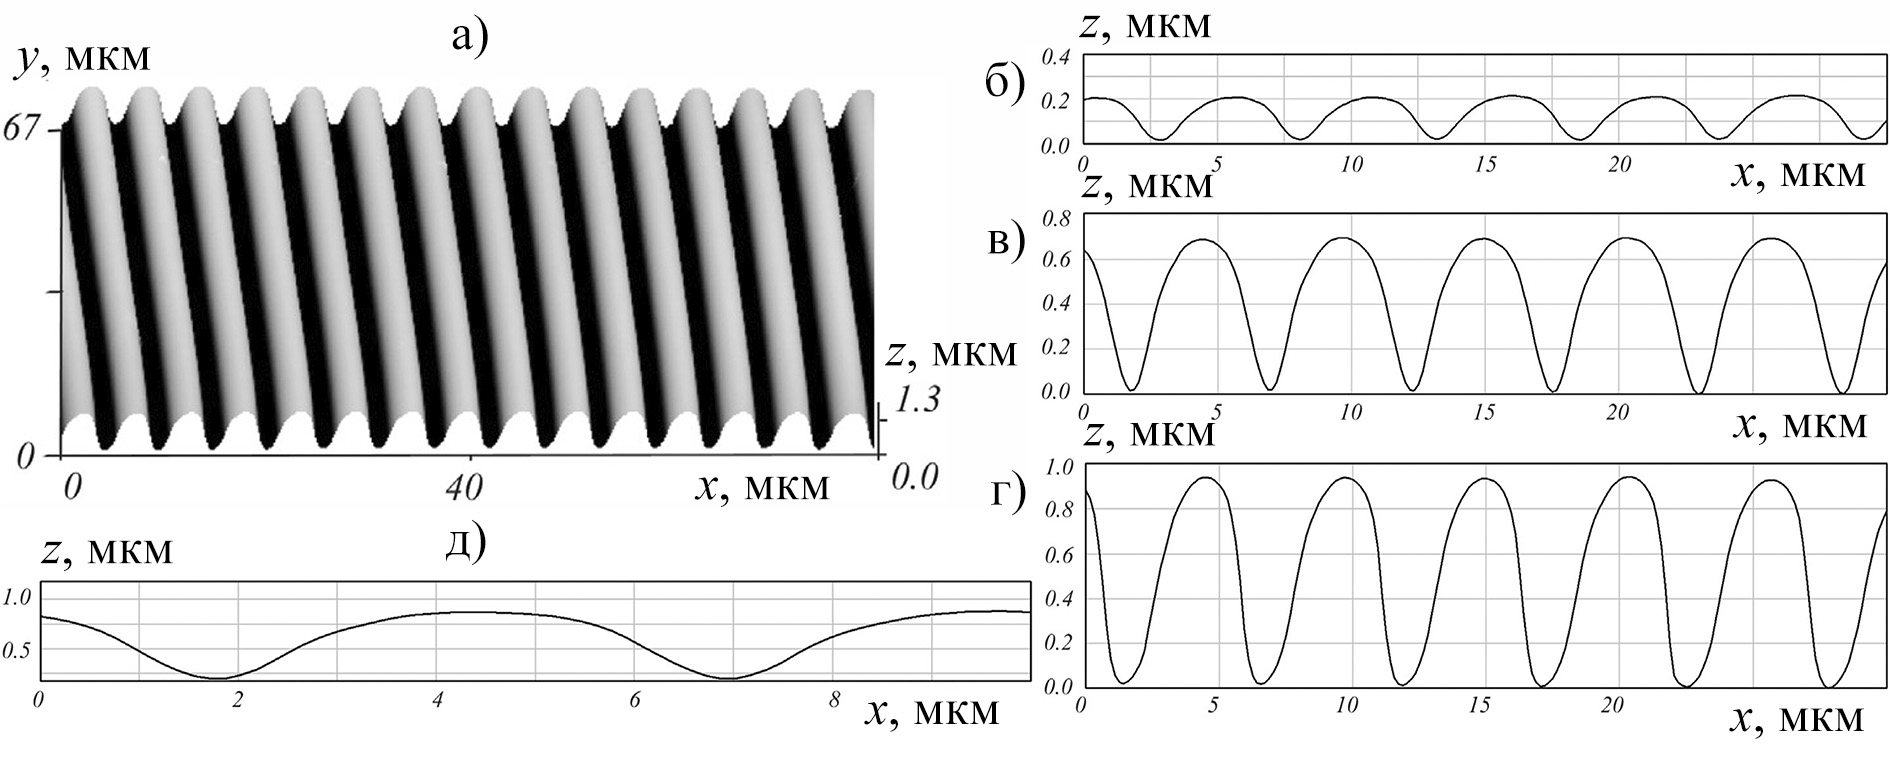
\includegraphics{jpg/DEBER_many_profiles_12pt_300}
%	\vspace{0.2em}
	\caption{Периодические профили, полученные методом СЭЛТР в слое ПММА толщиной 900 нм при экспонировании резиста ``в кадр''. Размеры кадра составляют 3$\times$3.9 мм$^2$, число линий в кадре -- 625, температура образца -- 160 $^\circ$C. а) --  Трехмерное изображение; б), в), г) -- профили, полученные при дозах экспонирования 0.05, 0.2 и 0.87 мкКл/см$^2$, соответственно, д) -- изображение профиля в) в масштабе 1:1~\cite{Bruk_2016_mee}.}
	\label{fig:DEBER_many_profiles}
\end{figure}

\underline{\textbf{Вторая глава}} посвящена описанию существующих моделей и методов моделирования основных процессов, протекающих при СЭЛТР. Некоторые процессы являются достаточно хорошо изученными -- например, в настоящее время существуют различные подходы к описанию упругого и неупругого рассеяния, и наиболее современные из них обеспечивают высокую точность моделирования~\cite{Czyzewski_mott_cs, Ciappa_2010, Valentin2012_Si}. В то же время, некоторые процессы являются изученными относительно слабо -- например, для описания процесса электронно-стимулированных разрывов полимерных молекул существует общий подход, основанный на анализе распределения выделившейся в резисте энергии~\cite{Greeneich1979_Mf_Mn}, и разработанная на его основе микроскопическая модель разрывов~\cite{Stepanova_2006} может применяться только для температур вблизи комнатной. В отдельную группу можно отнести процессы диффузии мономера в слое резиста и растекания резиста -- для их описания существуют относительно простые и в то же время достаточно точные методы~\cite{Vrentas_free_volume, Fragala_3_diffusion, Karlsson2001_diffusion, Leveder_2010, Kirchner_reflow}, однако их использование в исходном виде представляется невозможным в силу неоднородного профиля молекулярной массы резиста в методе СЭЛТР. Наконец, кинетические модели цепной деполимеризации резиста, описывающие изменение молекулярной массы резиста, требуют задания различных констант (как минимум, константы инициирования деполимеризации и средней длины цепи деполимеризации), значения которых приведены в литературе лишь для случаев простой термической деполимеризации (не являющейся электронно-стимулированной)~\cite{Boyd_3, Mita_PMMA_zip_lengths_T}. Все вышесказанное указывает на необходимость доработки большинства существующих подходов для их применения при моделировании метода СЭЛТР.

В \underline{\textbf{третьей главе}} приводятся методы, которые были использованы при разработке и верификации модели процесса СЭЛТР. В качестве резиста в разработанной модели использовался полиметилметакрилат (ПММА), в качестве материала подложки -- кремний. Для моделирования рассеяния электронного луча в резисте и подложке был использован алгоритм Монте-Карло с моттовскими сечениями упругого рассеяния~\cite{Czyzewski_mott_cs}:
\begin{equation}
	\frac{d \sigma_{e l}}{d \Omega}=|f(\theta)|^2+|g(\theta)|^2,
\end{equation}
где $f(\theta)$ и $g(\theta)$ -- амплитуды рассеяния, соответствующими параллельному и антипараллельному направлению спина электрона относительно его направления движения, и сечениями неупругого электрон-электронного рассеяния, рассчитанными из диэлектрической функции:
\begin{equation}
	\frac{d \sigma_{e-e}^{-1}}{d \hbar \omega}=\frac{1}{\pi E a_0 n} \int_{k_{-}}^{k_{+}} \operatorname{Im}\left[\frac{-1}{\varepsilon(q, \omega)}\right] \frac{d q}{q},
\end{equation}
где
\begin{equation}
	q_{\pm}=\frac{\sqrt{2 m}}{\hbar}(\sqrt{E} \pm \sqrt{E-\hbar \omega}),
\end{equation}
$E$ -- энергия налетающего электрона, m -- масса электрона, $a_0$ -- боровский радиус, $n$ -- концентрация рассеивающих центров в веществе. Для ПММА функция потерь энергии $\operatorname{Im}\left[\frac{-1}{\varepsilon(q, \omega)}\right]$ определялась на основе диэлектрической функции Мермина~\cite{Mermin}, для кремния -- как сумма функций потерь энергии отдельных осцилляторов~\cite{Valentin2012_Si}. Для повышения точности при моделировании рассеяния низкоэнергетических электронов в ПММА также учитывалось электрон-фононное и электрон-поляронное взаимодействие~\cite{Ciappa_2010}.

Для описания электронно-стимулированных разрывов молекул ПММА при повышенной температуре была разработана оригинальная микроскопическая модель. В качестве приводящих к разрыву полимерных молекул рассматривались акты электрон-электронного рассеяния, и для моделирования электронно-стимулированных разрывов молекул была введена вероятность разрыва при электрон-электронном рассеянии $p_s$. При заданной вероятности разрыва $p_s$ акты электрон-электронного взаимодействия, приводящие к разрыву молекул, моделировались методом Монте-Карло:
\begin{equation} \label{eq:MC_9}
	\begin{aligned}
		\xi < p_s & \Rightarrow \text{разрыв молекулы} \\
		\xi \geq p_s & \Rightarrow \text{нет разрыва}
	\end{aligned}
\end{equation}
где $\xi$ -- случайное число из промежутка [0, 1). Значение $p_s$ для различных температур было определено путем моделирования эксперимента по определению радиационно-химического выхода разрывов $G_s$. $G_s$ определяется как число разрывов,  происходящих при выделении в нем энергии 100 эВ, и может быть определено экспериментально на основе среднечисловых значений молекулярной массы полимера до и после экспонирования ($M_n$ и $M_f$, соответственно):
\begin{equation}
	\begin{aligned}
		G_s = n_{\text{разрывов}} / 100 \text{ эВ} & - \text{теоретически} \\
		G_s: M_f = \frac{\displaystyle M_n}{1 + \frac{\displaystyle G_s \epsilon}{\displaystyle 100 \rho N_A}}& - \text{экспериментально},
	\end{aligned}
\end{equation}
где $\epsilon$ -- энергия, выделившаяся в единице объема резиста, $\rho$ -- плотность резиста, $N_A$  -- постоянна Авогадро.

Моделирование слоя резиста размерами 100$\times$100$\times$500 нм$^3$ производилось на основе модели идеальной цепи~\cite{Han_2002}, и дальнейшее сопоставление промоделированных актов электрон-электронного рассеяния конкретным мономерам позволило промоделировать распределение молекулярной массы проэкспонированного резиста при различных значениях $p_s$. Так для каждой температуры было подобрано значение $p_s$, обеспечивающее соответствие между промоделированным и экспериментальным~\cite{Charlesby_1964_Gs} значением радиационно-химического выхода разрывов. На рис.~\ref{fig:P_s} приведены температурные зависимость $p_s$, вычисленные при моделировании $G_s$ и непосредственно на основе числа разрывов и выделившейся в резисте энергии. Различие между ними указывает на целесообразность моделирования распределения молекулярной массы для определения $p_s$.
\begin{figure}[t]
	\centering
	\includegraphics[width=0.6\linewidth]{G_value/G_s_300}
	\caption{Зависимость вероятности разрыва $p_s$ молекулы ПММА при электрон-электронном взаимодействии от температуры $T$ резиста в диапазоне температур 0--200$^\circ$C.\vspace{1.5em}}
	\label{fig:P_s}
\end{figure}

Для моделирования электронно-стимулированной цепной деполимеризации ПММА в условиях метода СЭЛТР была использована кинетическая модель термической деполимеризации при инициировании активных центров деполимеризации в произвольных точках молекулы~\cite{Boyd_3}. С учетом процессов инициирования деполимеризации, распространения активного центра деполимеризации вдоль молекулы и его исчезновения эта модель может быть сформулирована в виде системы дифференциальных уравнения на моменты функции распределения молекулярной массы резиста:
\begin{equation} \label{eq:moment_equation}
	\frac{d M_i}{d t}=k_s\left(\frac{2}{i+1}-1\right) M_{i+1}+\frac{d M_0}{d t}-k_s M_1 - \frac{i}{\gamma}\left(k_s M_i+\frac{d M_{i-1}}{d t}\right) \quad(i \geq 1),
\end{equation}
$k_s$ -- константа инициирования деполимеризации (число активных центров деполимеризации, появившихся за 1 с, приходящееся на один мономер), $1/\gamma$ -- средняя длина цепи деполимеризации, $M_i$ -- момент функции распределения порядка $i$ ($P_n$ -- число полимерных молекул степени полимеризации $n$):
\begin{equation}
	M_i=\sum_{n=2}^{\infty} n^i P_n.
\end{equation}

Данная система решалась численно в предположении, что распределение молекулярной массы резиста описывается функцией распределения Шульца-Цимма~\cite{Schulz-Zimm_distribution} для каждой ячейки резиста размерами 100$\times$100$\times$5 нм$^3$. При определении $k_s$ в каждой ячейке считалось, что число активных центров деполимеризации, появившихся за 1 с в ячейке, равно числу разрывов полимерных молекул, промоделированных с помощью вышеописанного подхода, число мономеров в ячейке определялось на основе плотности и молярной массы ПММА. Такой подход позволил промоделировать локальное изменение распределения молекулярной массы ПММА в ходе экспонирования в процессе СЭЛТР. (рис.~\ref{fig:Mn_hist})

\begin{figure}[t]
	\begin{center}
		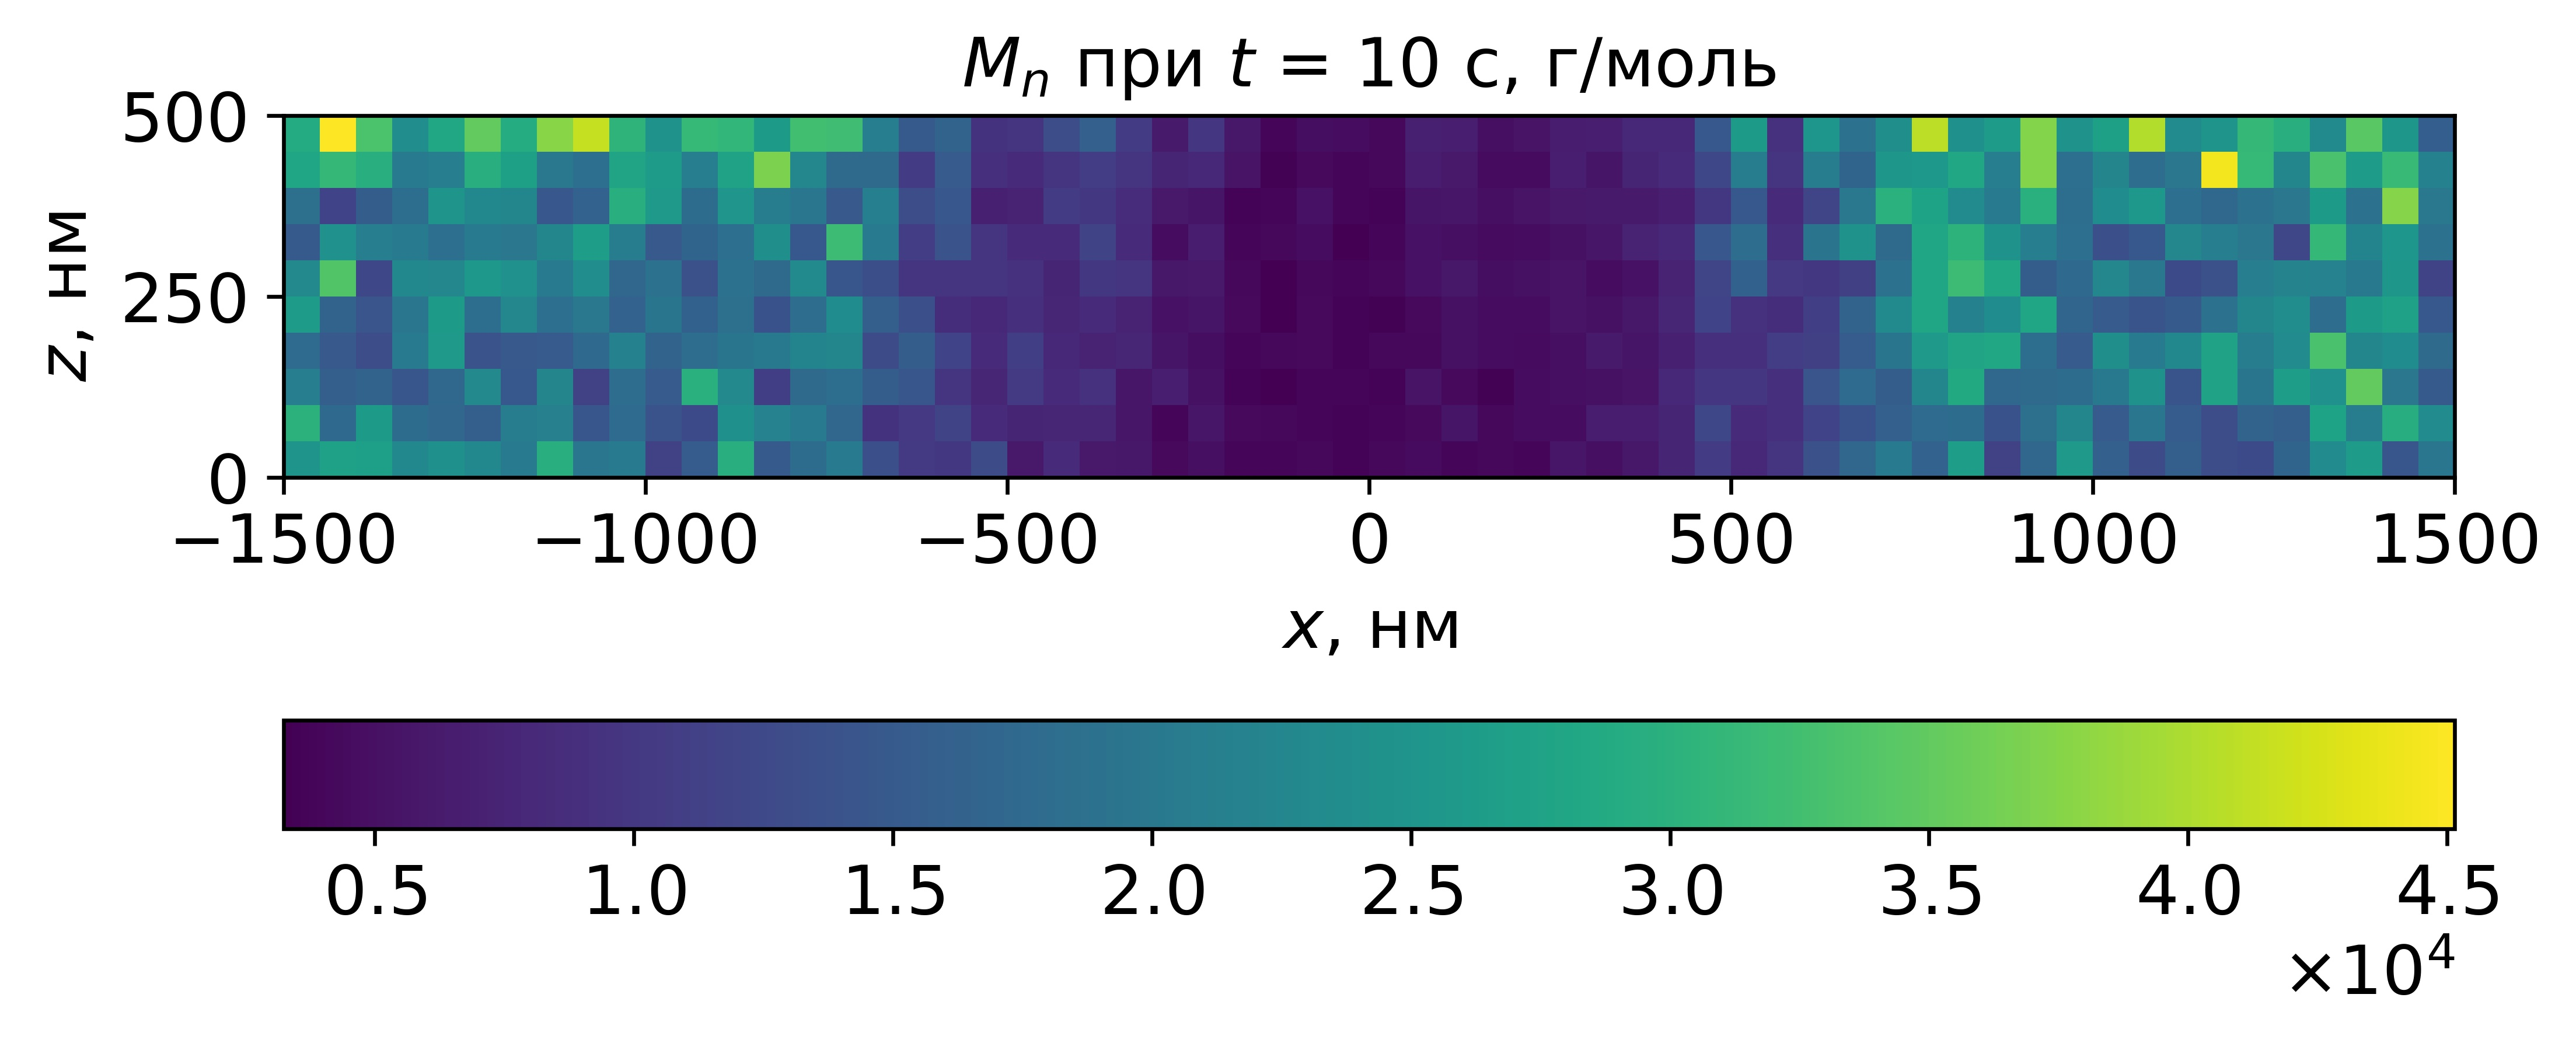
\includegraphics[width=0.7\linewidth]{MW/Mn_hist_10s_14} \\
		\vspace{-3.7em} \text{\hspace{-26em} a)} \vspace{2.7em} \\
		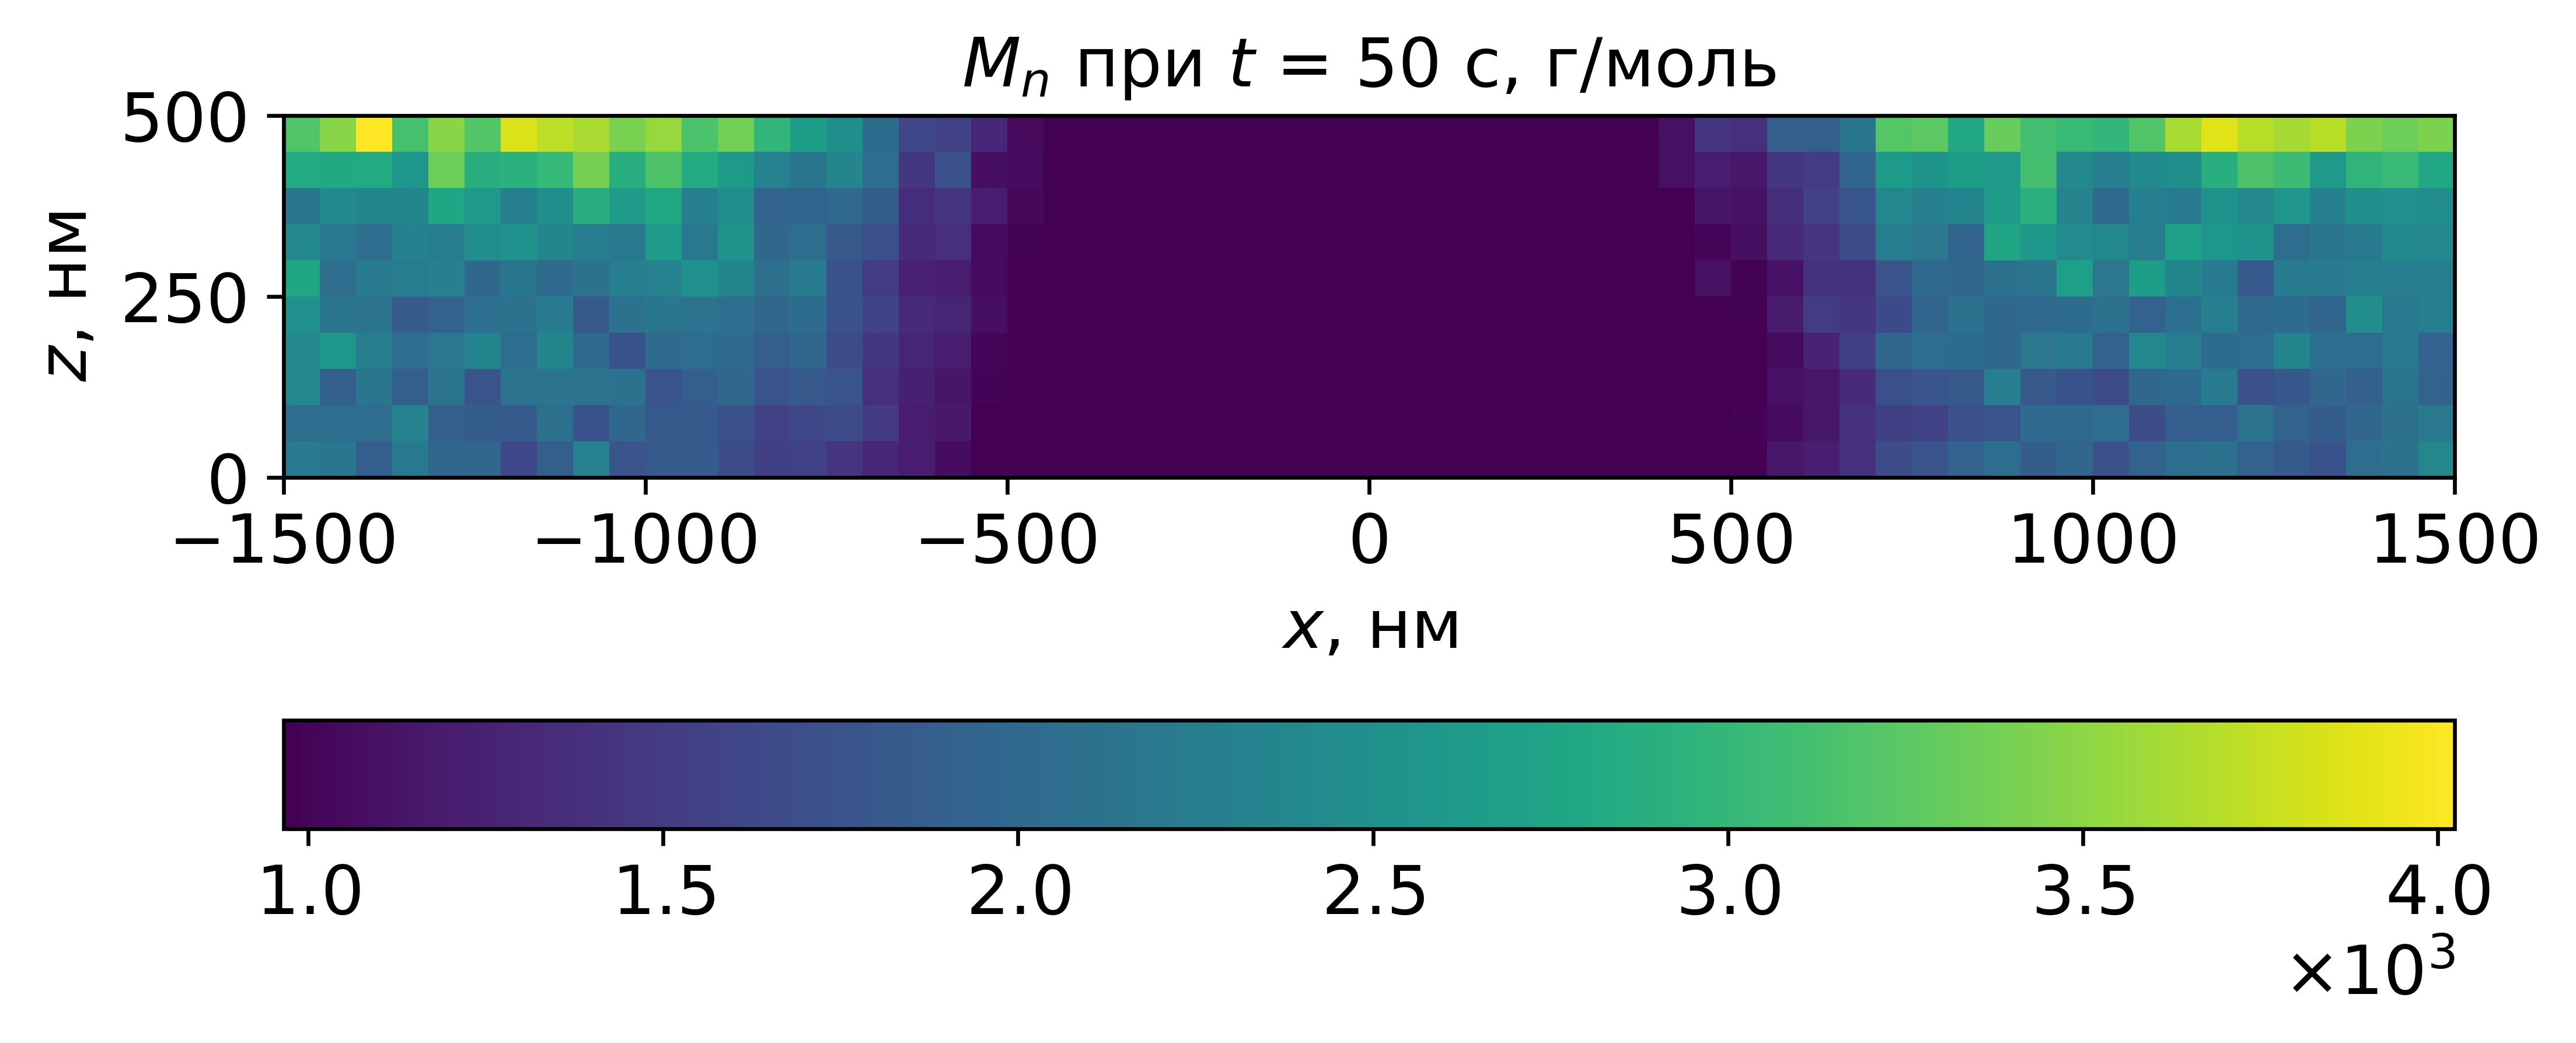
\includegraphics[width=0.7\linewidth]{MW/Mn_hist_50s_14} \\
		\vspace{-3.7em} \text{\hspace{-26em} б)} \vspace{3.7em} \\
	\end{center}
	\vspace{-2.5em}
	\caption{Моделирование распределения среднечисловой молекулярной массы ПММА марки 950К при его экспонировании электронным лучом «в кадр», с расстоянием между линиями 3 мкм. На рис. показано распределение локальной молекулярной массы резиста в пределах одной линии. Плотность тока на единицу длины линии составляет около 3 нА/см, начальная энергия электронов в пучке – 20 кэВ, толщина слоя ПММА -- 500 нм, температура образца -- 150 $^\circ$C. Время экспонирования составляет 10 с (а) и 50 с (б).}
	\label{fig:Mn_hist}
\end{figure}

Моделирование локального распределения молекулярной массы ПММА сделало возможным определение локального значений коэффициента диффузии мономера, образующегося в слое ПММА в результате деполимеризации, $D$, а также вязкости резиста $\eta$ на основе экспериментальных значений и зависимостей, приведенных в работах~\cite{Fragala_3_diffusion, aho2008measurement_WLF, Berens_diffusion_Mn, Leveder_2010, Bueche_3p4_1p4}. Моделирование диффузии путем численного решения уравнения диффузии показало, что в условиях метода СЭЛТР коэффициент диффузии за первые секунды экспонирования снижается до значений, при которых время диффузии мономера из слоя толщиной в несколько сотен нанометров составляет менее 1 с. Таким образом, в дальнейшем считалось, что мономер, образовавшийся в процессе деполимеризации мгновенно покидает объем травления, что приводит к образованию микрополостей в слое ПММА.

Для моделирования растекания ПММА с неоднородным профилем вязкости использовался численный подход на основе метода конечных элементов~\cite{Brakke_SE}. В нем процесс растекания какого-либо тела рассматривается как процесс эволюции его поверхности, направленный на уменьшение поверхностной энергии, и при этом различие коэффициентов вязкости различных участков тела может быть учтено за счет задания различных значений подвижности вершин поверхности. Для определения соотношения, связывающего вязкость тела и подвижность вершин его поверхности было проведено моделирование растекания прямоугольных решеток с постоянным значением вязкости аналитическим~\cite{Leveder_2010} и численным методом. Для значений коэффициента вязкости в диапазоне 10$^2$--10$^6$ Па с были подобраны значения подвижности вершин поверхности решетки, обеспечивающие соответствие результатами, полученными обоими методами~(рис.~\ref{fig:C_gamma}). В результате было установлено, что подвижность вершин поверхности $\mu$ может быть рассчитана из вязкости резиста $\eta$ по формуле
\begin{equation}
	\mu \approx \frac{26.14}{\eta}.
\end{equation}

Полученная зависимость позволяет рассчитывать локальную подвижность вершин резиста с неоднородным профилем вязкость, определенным с помощью вышеописанного подхода.

\begin{figure}[h]
	\begin{center}
		\includegraphics[width=0.5\textwidth]{reflow/С_gamma_12}
	\end{center}
	\vspace{-1.2em}
	\caption{Полученная зависимость подвижности вершин поверхности ПММА от его вязкости.}
	\label{fig:C_gamma}
\end{figure}

Для моделирования растекания резиста моделируется пилообразная структура, в которой объем ``зубьев'' равен суммарному объему микрополостей в резисте (рис.~\ref{fig:reflow_surface}).

\begin{figure}[h]
	\begin{minipage}{0.48\textwidth}
		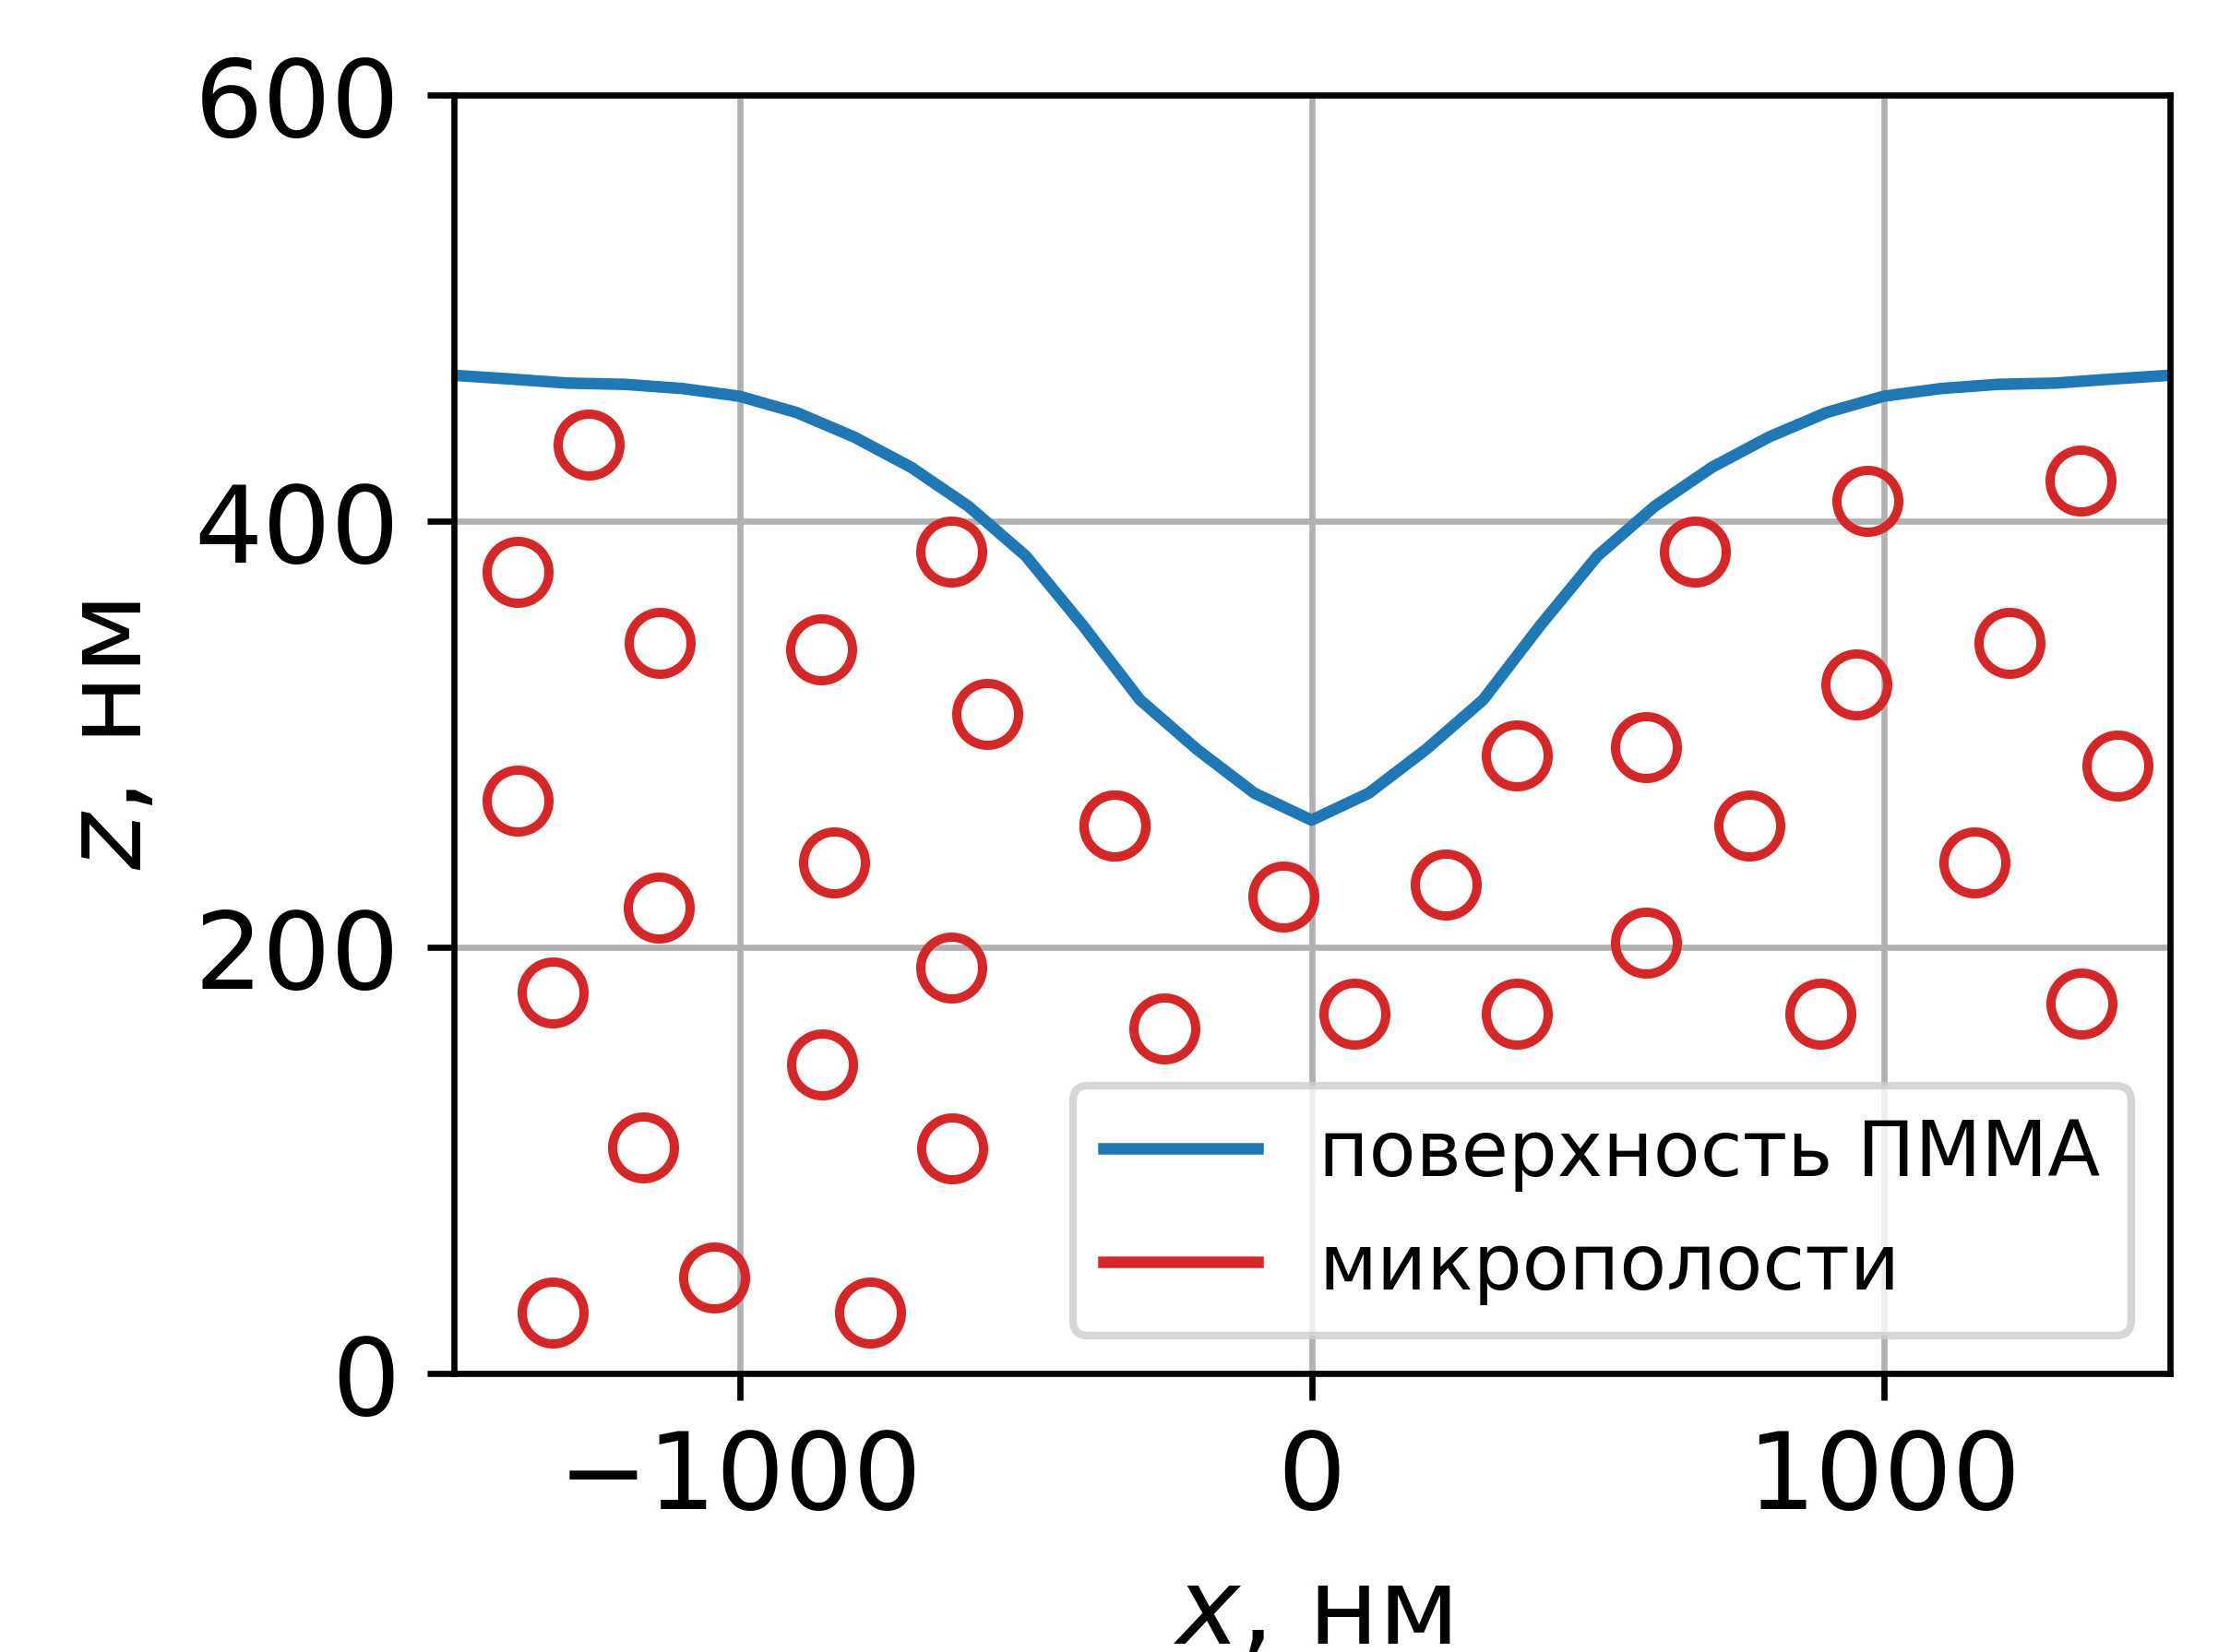
\includegraphics[width=0.9\linewidth]{reflow/reflow_initial_circles_14} \\
		\vspace{-28.5ex} \\ \text{\hspace{0em} a}) \\ \vspace{28.5ex}
	\end{minipage}
	\begin{minipage}{0.48\textwidth}
		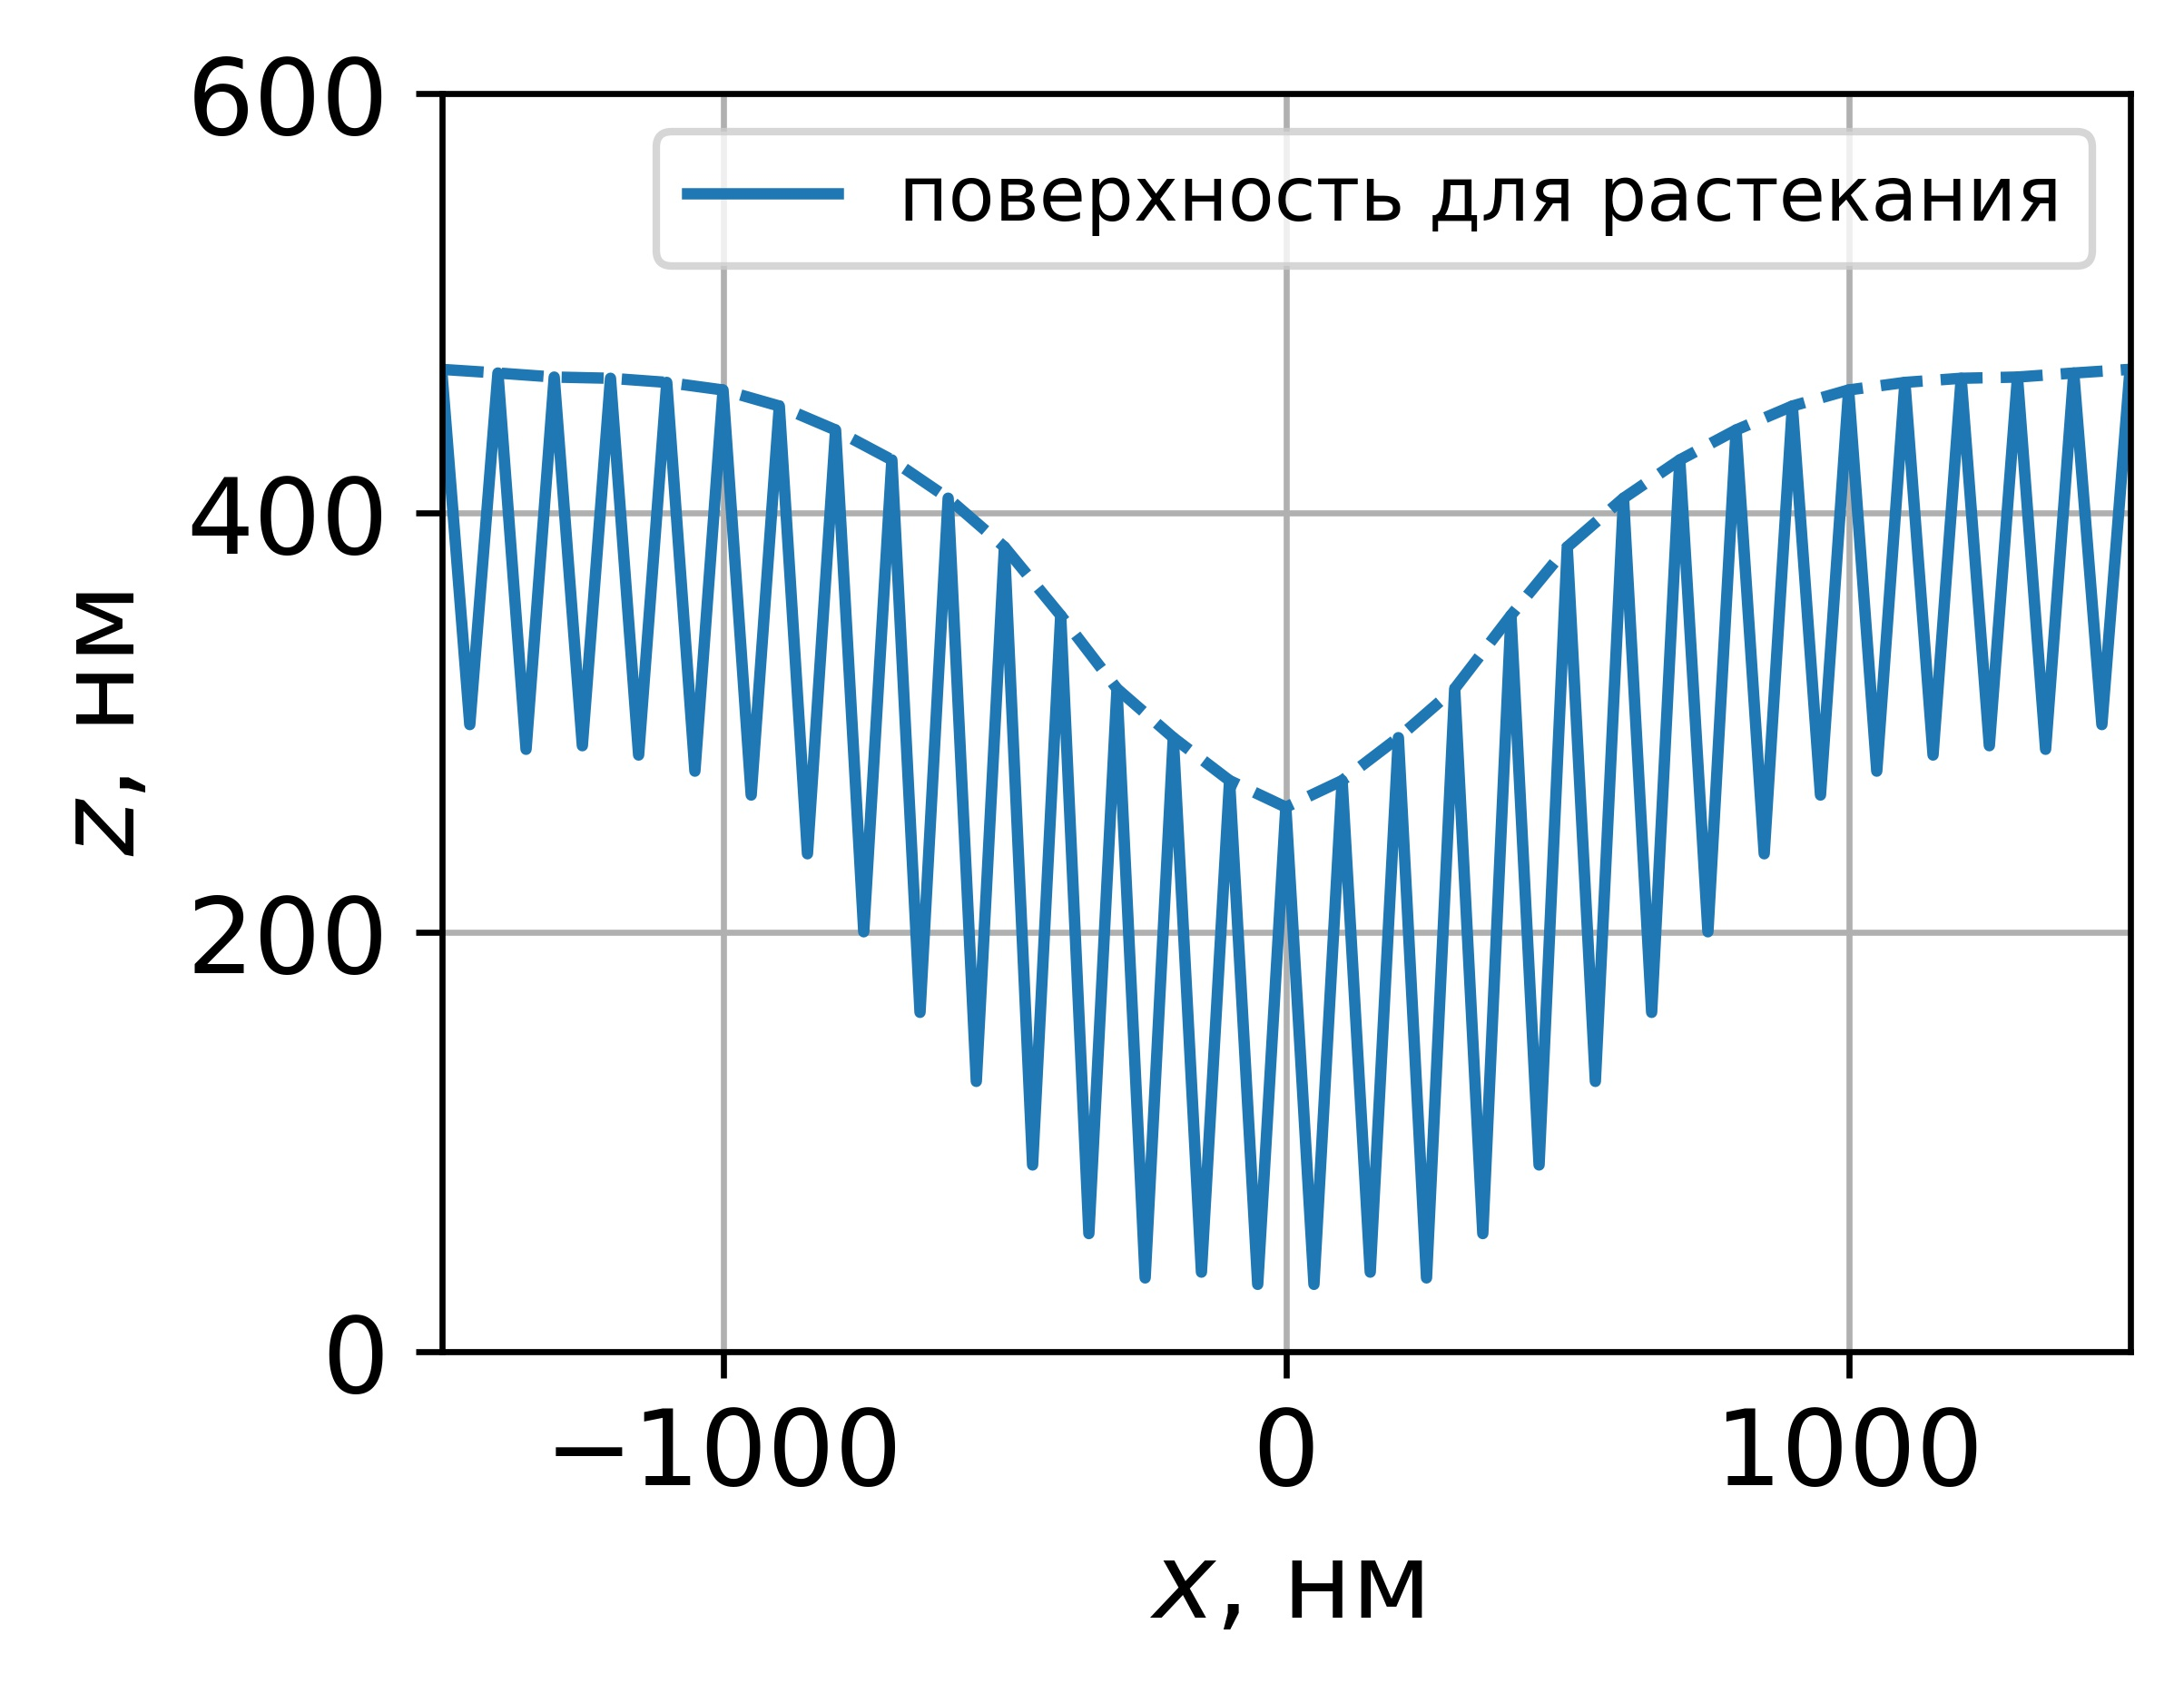
\includegraphics[width=0.9\linewidth]{reflow/reflow_fin_14} \\
		\vspace{-28.5ex} \\ \text{\hspace{-0.1em} б}) \\ \vspace{28.5ex}
	\end{minipage}
	\vspace{-3.5em}
	\caption{Иллюстрация подхода к моделированию растекания слоя ПММА со внутренними микрополостями.}
	\label{fig:reflow_surface}
\end{figure}

Вышеописанные модели отдельных процессов, протекающих при СЭЛТР были использованы для разработки алгоритма моделирования конечного профиля линии, получаемой этим методом. Для этого все время экспонирования разбивалось на промежутки величиной 1 с, и в течение каждого промежутка последовательно производились следующие действия:
\begin{enumerate}
	\item Моделирование рассеяния электронного пучка в ПММА и подложке;
	\item Моделирование разрывов молекул ПММА;
	\item Вычисление локальной молекулярной массы и вязкости ПММА;
	\item Вычисление объемов образовавшихся в ПММА микрополостей на основе концентрации разрывов и значения средней длины цепи деполимеризации;
	\item Преобразование слоя ПММА со внутренними микрополостями в пилообразную структуру;
	\item Моделирование растекания пилообразной структуры;
	\item Определение нового положение вершин поверхности слоя ПММА.
\end{enumerate}

По истечении времени экспонирования также моделировалось растекание слоя ПММА при его охлаждения до температуры, при которой процессы растекания перестают протекать заметным образом (было установлено, что эта температура составляет около 80$^\circ$C).

Для верификации разработанной модели методом СЭЛТР были получены периодические структуры в слое ПММА (марки 950K) с начальной толщиной 500 нм на кремниевой подложке. Для экспонирования резиста использовался электронный микроскоп CAMSCAN S-4, который был модифицирован для возможности нагрева образца. Давление в камере микроскопа находилось на уровне 10$^{\text{-5}}$ мбар, энергия электронов в пучке составляла 20 кэВ, диаметр пучка -- около 600 нм.

Экспонирование резиста проводилось ``в кадр'' с размером кадра 2.4$\times$1.9 см$^\text{2}$, число линий в кадре равнялось 625. Ток экспонирования $I_{exp}$ находился в диапазоне 4.56--5.62 нА, время экспонирования $t_{exp}$ варьировалось от 100 до 200 с, таким образом, доза экспонирования на единицу длины линии $D_l$ находилась в диапазоне 3.00--3.69 нКл/см. Температура образцов при экспонировании $T$ варьировалась от 130 до 150~$^\circ$C, скорость охлаждения образца после экспонирования составляла около 0.2~$^\circ$C/с, скорость охлаждения подложки после экспонирования -- около 0.2 $^\circ$С/с. При снижении температуры образца до 50~$^\circ$C он извлекался из камеры микроскопа. Профили линий были получены методом атомно-силовой микроскопии с помощью микроскопа Nanopics 2100.

Для снижения требуемого машинного времени моделирование проводилось для участка одной линии длиной 100 нм, и влияние соседних линий учитывалось за счет использования зеркальных граничных условий. Число разрывов, локальная молекулярная и объем микрополостей вычислялись для областей размерами 100 нм $\times $100 нм $\times$ 5 нм (по осям $x$, $y$ и $z$, соответственно).

Для учета стохастической природы алгоритма моделирования здесь и далее конечный промоделированный профиль получался за счет усреднения 100 отдельно промоделированных профилей. Сравнение экспериментальных и промоделированных профилей приведено на рис.~\ref{fig:DEBER_4_profiles}. Высокая степень воспроизведения экспериментальных профилей указывает на достоверность разработанной модели метода СЭЛТР.

Было установлено, что при при описанных выше параметрах экспонирования средняя длина цепи деполимеризации остается постоянной на протяжении первых 100 с процесса, и ее значения составляют 100 и 150 для температур 130~$^\circ$C и 150~$^\circ$C, соответственно. При дальнейшем экспонировании средняя длина цепи деполимеризации снижается, и на временном промежутке 100--200 с ее значения составляют 70 и 30 для температур 130~$^\circ$C и 150~$^\circ$C, соответственно. Следует отметить, что по порядку величины эти значения согласуется со значениями, рассчитанными на основе констант процессов, протекающих при деполимеризации резиста~\cite{Mita_PMMA_zip_lengths_T}.

\begin{figure}[h!]
	\begin{minipage}{0.48\textwidth}
		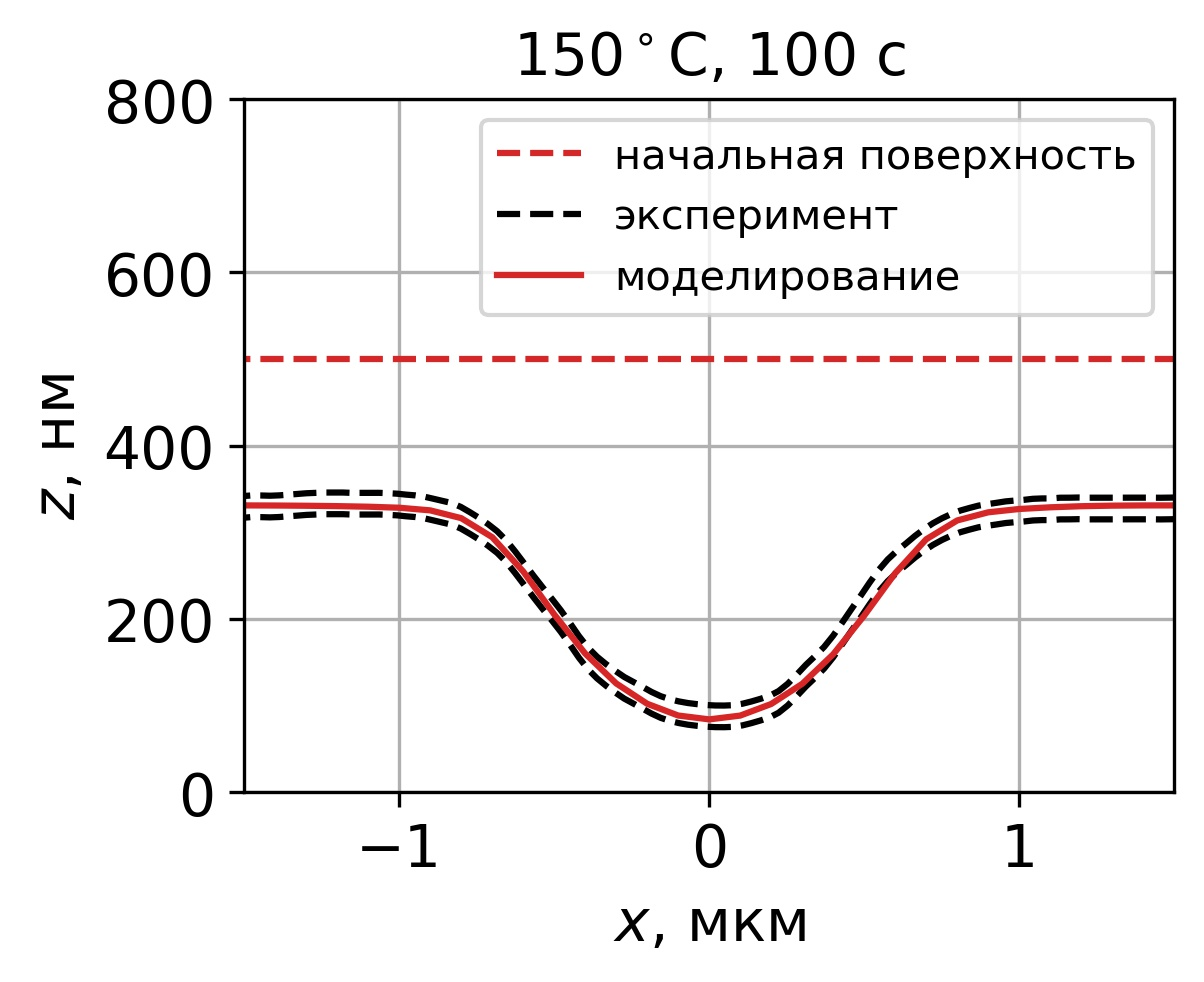
\includegraphics[width=0.9\linewidth]{DEBER_verification/150C_100s_14_dPMMA_um_300dpi} \\
		\vspace{-13em} \\ \text{\hspace{0em} a}) \\ \vspace{13em}
	\end{minipage}
	\begin{minipage}{0.48\textwidth}
		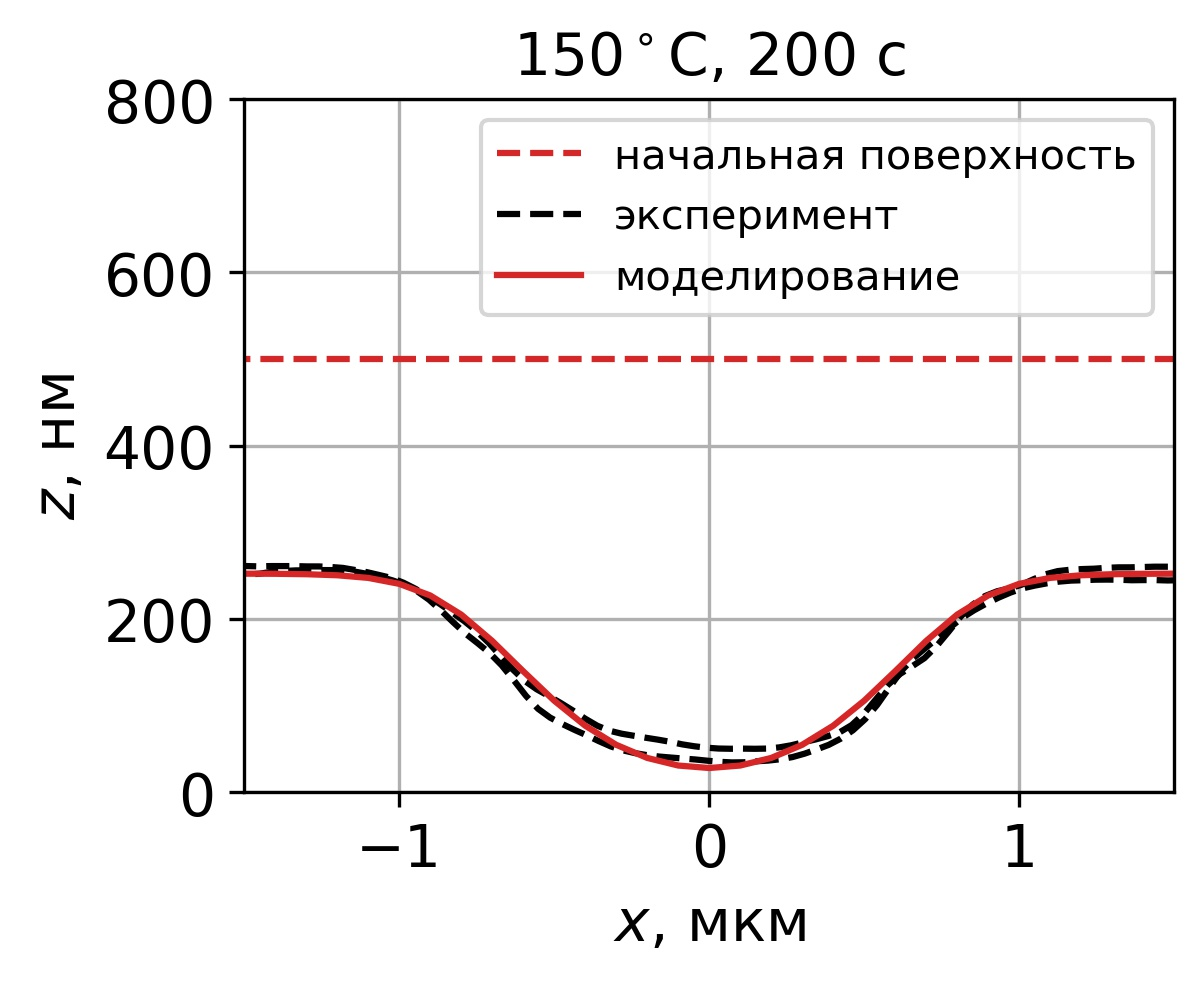
\includegraphics[width=0.9\linewidth]{DEBER_verification/150C_200s_14_dPMMA_um_300dpi} \\
		\vspace{-13em} \\ \text{\hspace{-0.1em} б}) \\ \vspace{13em}
	\end{minipage}
	
	\vspace{-3.5em}
	
	\begin{minipage}{0.48\textwidth}
		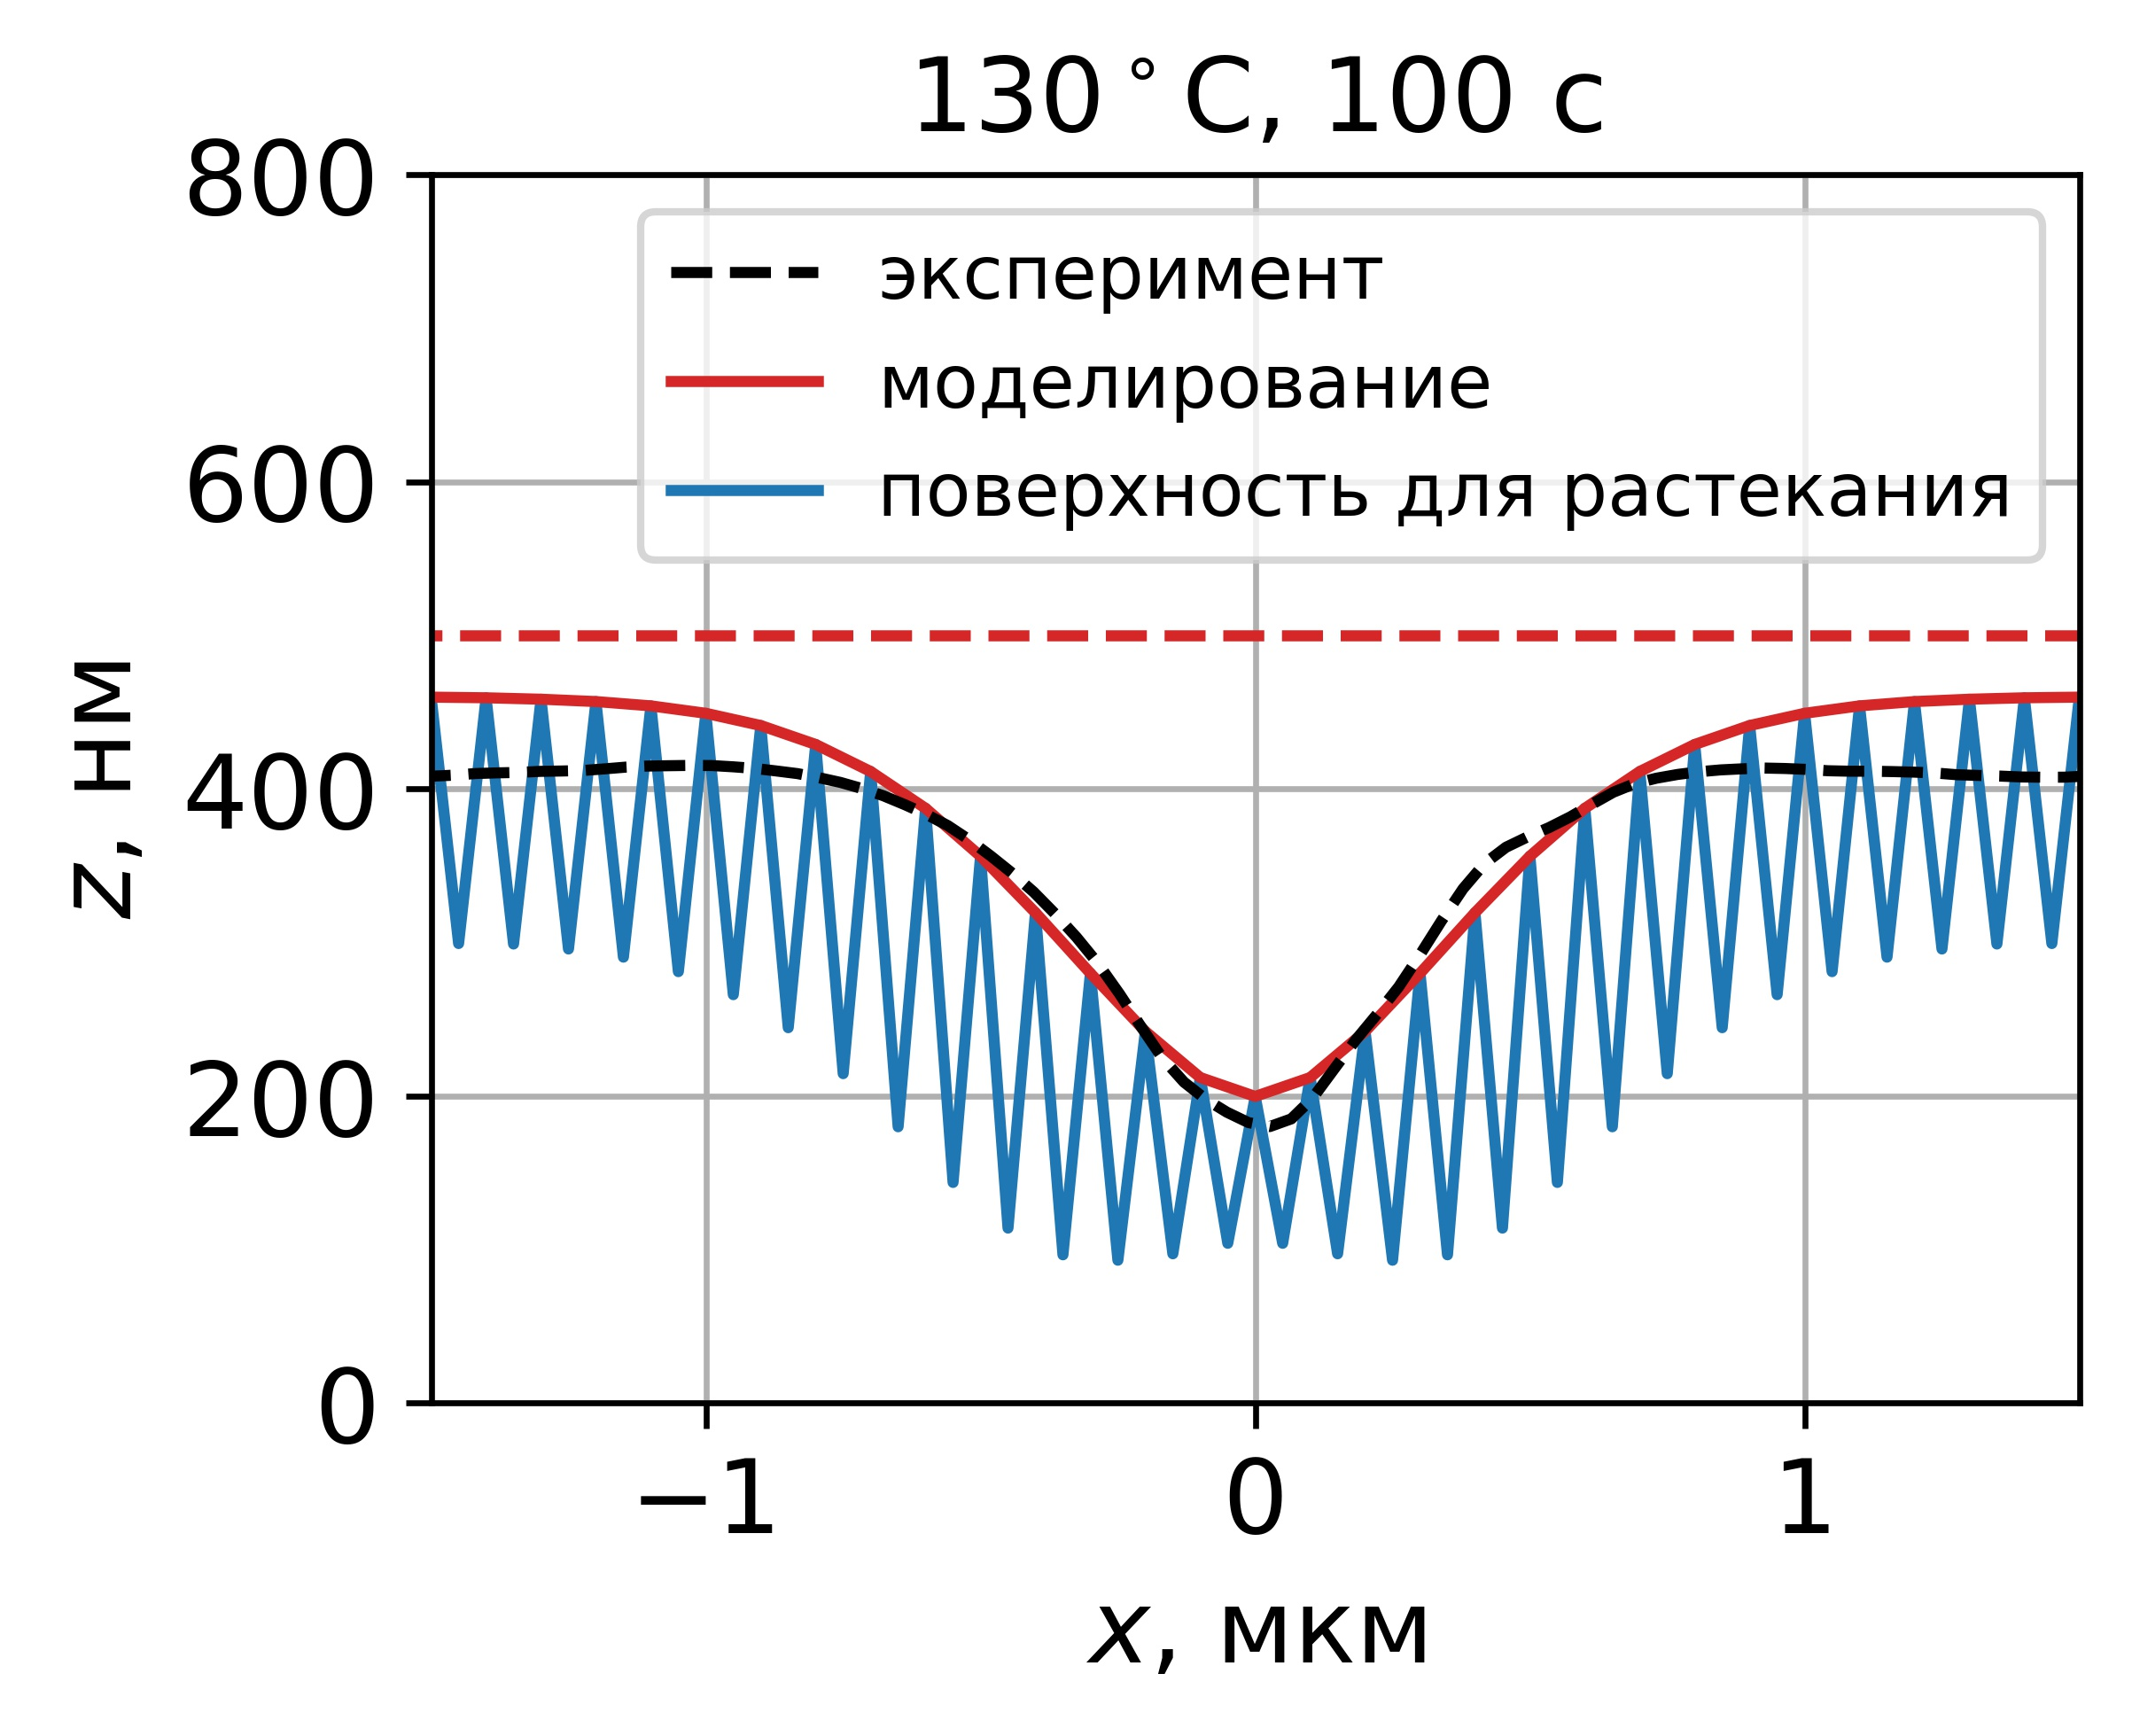
\includegraphics[width=0.9\linewidth]{DEBER_verification/130C_100s_14_inner_dPMMA_um_300dpi} \\
		\vspace{-13em} \\ \text{\hspace{0em} в}) \\ \vspace{13em}
	\end{minipage}
	\begin{minipage}{0.48\textwidth}
		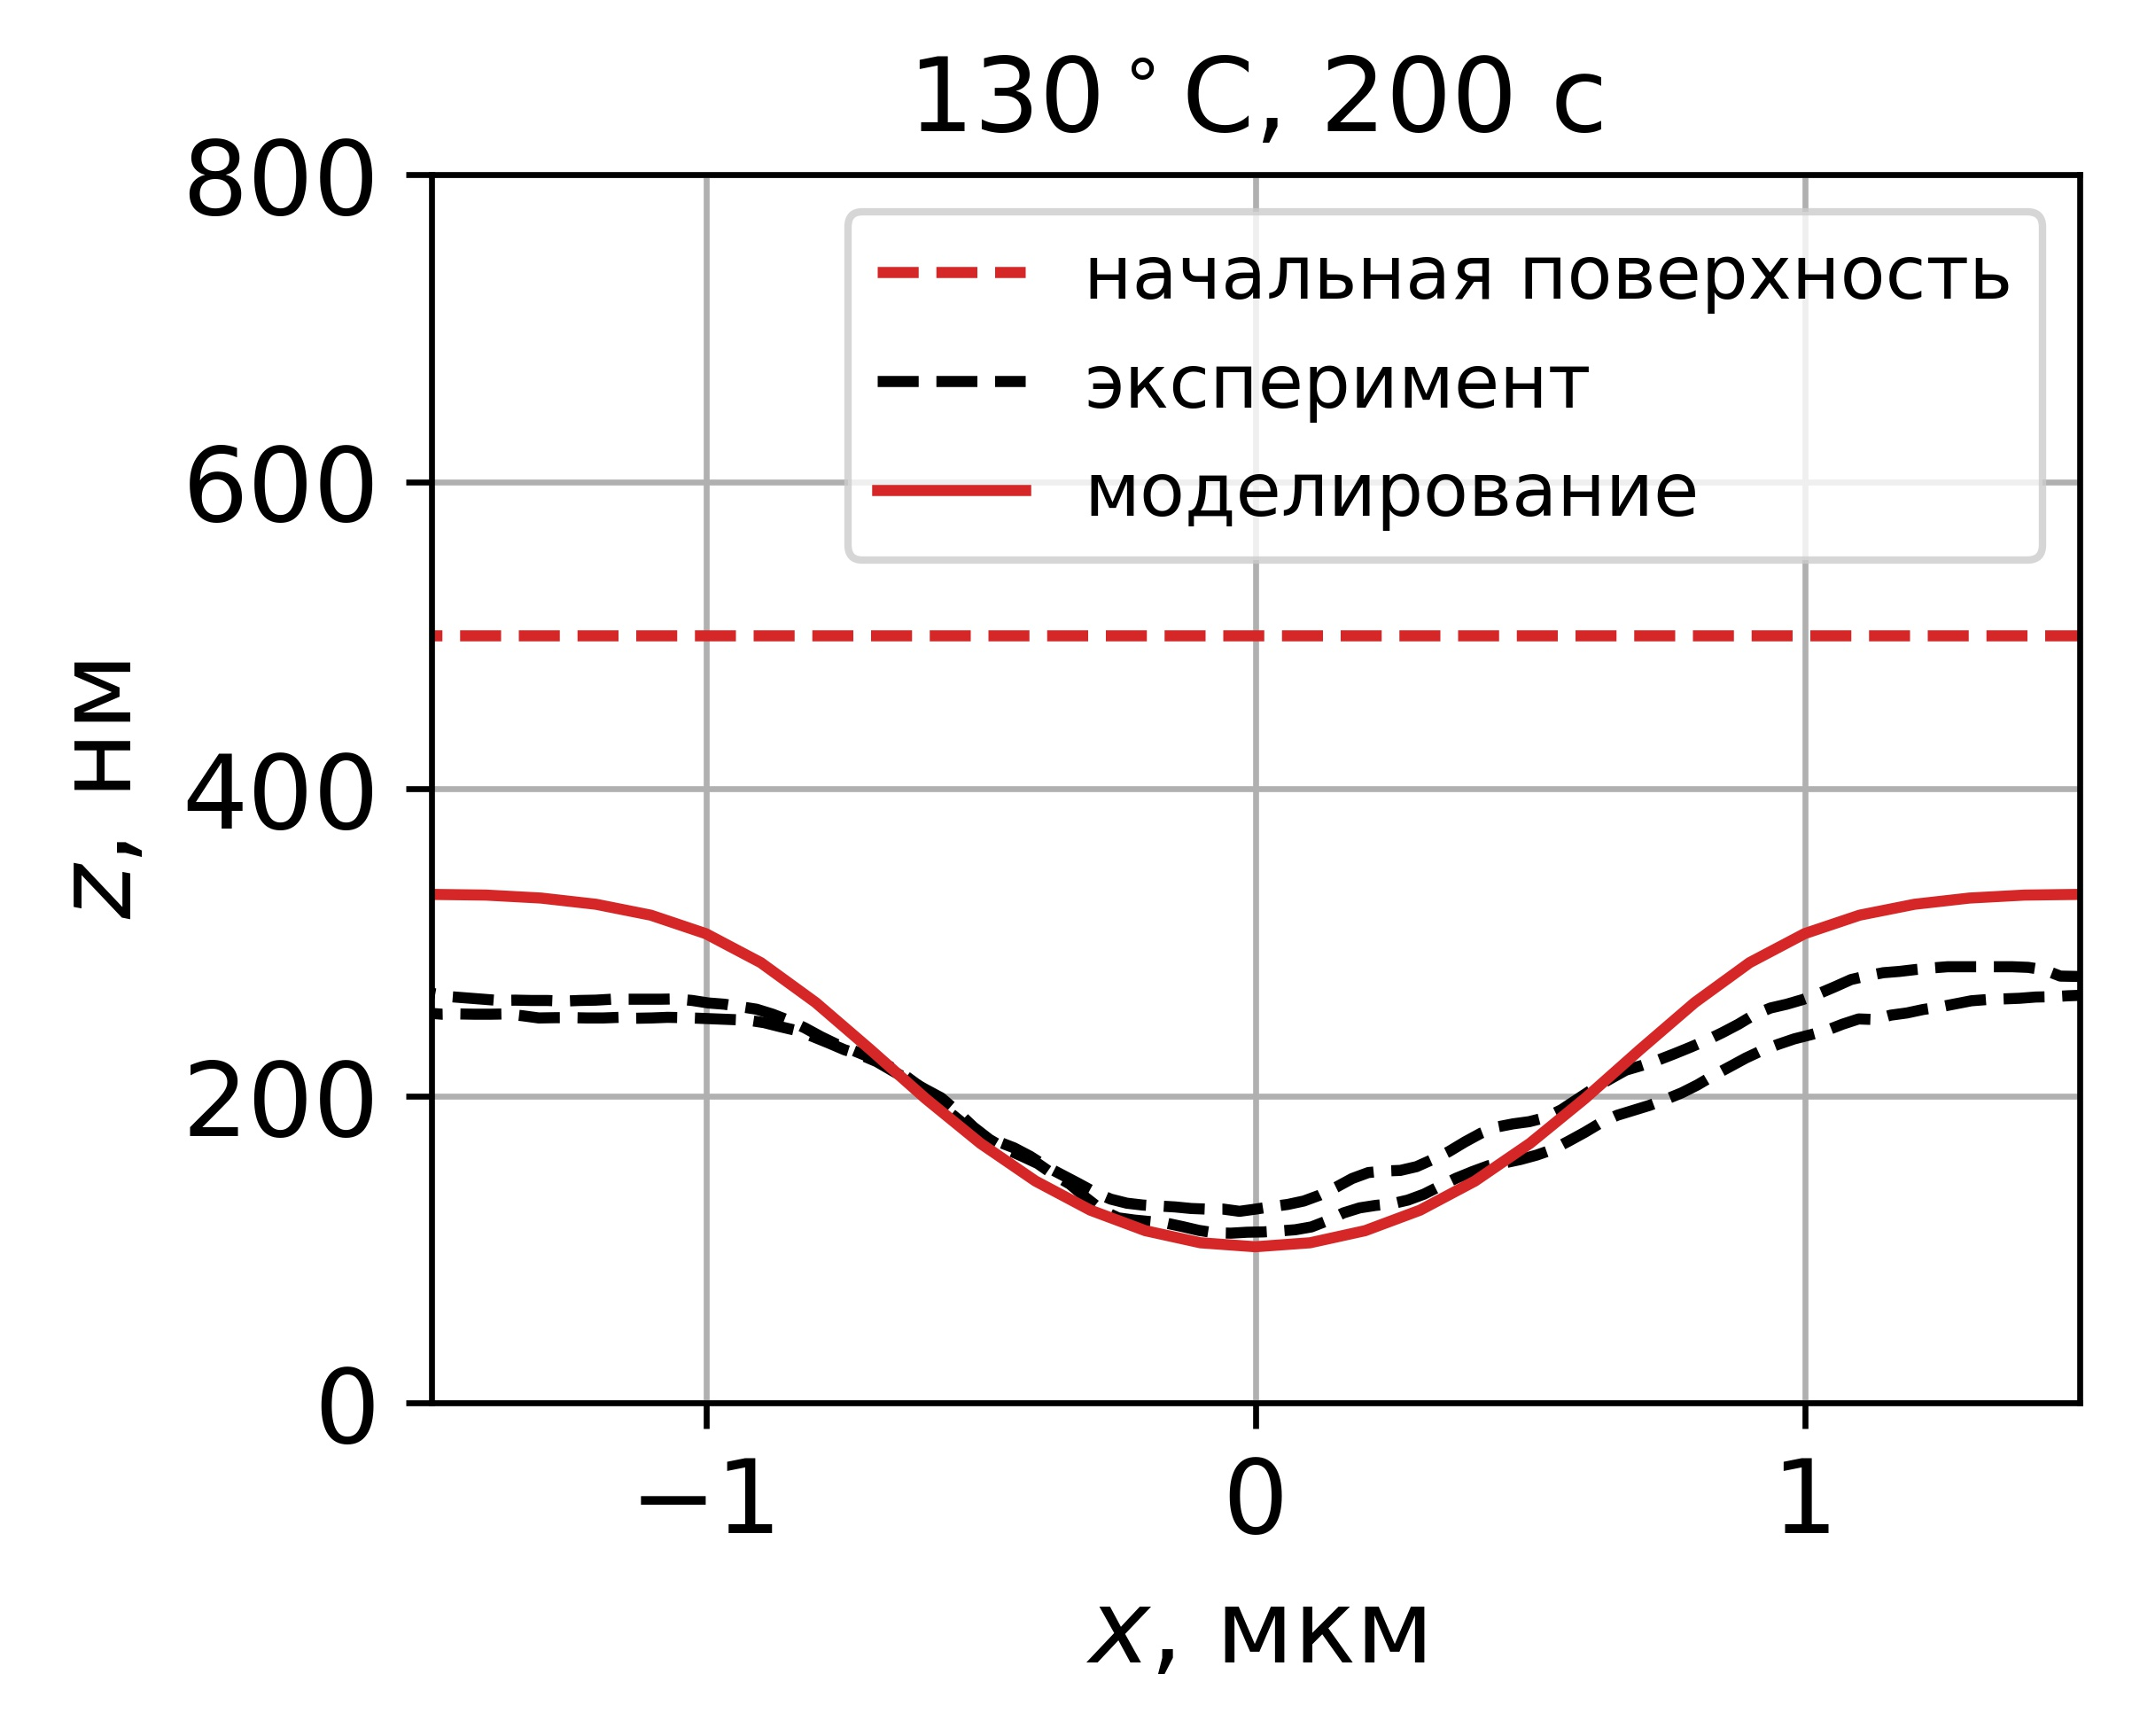
\includegraphics[width=0.9\linewidth]{DEBER_verification/130C_200s_14_dPMMA_um_300dpi} \\
		\vspace{-13em} \\ \text{\hspace{-0.1em} г}) \\ \vspace{13em}
	\end{minipage}
	\vspace{-3em}
	\caption{Верификация разработанной модели процесс СЭЛТР -- сравнение экспериментальных и промоделированных профилей, полученных при различных параметрах экспонирования: a) $T$ = 150 $^\circ$C, $t_{exp}$ = 100 c, $D_l$ = 3.00 нКл/см; б) $T$ = 150 $^\circ$C, $t_{exp}$ = 200 c, $D_l$ = 3.37 нКл/см; в) $T$ = 130 $^\circ$C, $t_{exp}$ = 100 c, $D_l$ = 3.12 нКл/см; в) $T$ = 130 $^\circ$C, $t_{exp}$ = 200 c, $D_l$ = 3.69 нКл/см. Во всех случаях, энергия пучка составляет 20 кэВ, диаметр пучка -- около 600~нм, охлаждение описывается экспериментальной кривой охлаждения. Черная пунктирная линия обозначает профиль (или профили), полученные в эксперименте, красная пунктирная линия -- начальное положение поверхности ПММА, синяя линия -- пилообразную поверхность, использовавшуюся для моделирования растекания слоя ПММА со внутренними микрополостями.}
	\label{fig:DEBER_4_profiles}
	\vspace{1em}
\end{figure}

Было установлено, что при полном затягивании микрополостей внутри слоя ПММА на момент остывания образца среднеквадратичное отклонение высоты точек профиля составляет примерно от 0.5 до 3 нм со средним значением около 2 нм. Однако, при наличии микрополостей внутри слоя ПММА на момент остывания (образец, полученный при экспонировании в течение 100 С при температуре 130~$^\circ$C) среднеквадратичное отклонение точек в центре линии превышает 10 нм.

Разработанная модель процесса СЭЛТР позволяет определить влияние параметров экспонирования на результирующий профиль линии. В том числе, с помощью данной модели можно определить влияние флуктуаций параметров экспонирования на форму профиля.
Было установлено, что в качестве требований к стабильности параметров экспонирования в методе СЭЛТР могут быть приняты максимальные значения флуктуации энергии пучка, тока экспонирования и температуры образца, составляющие примерно 0.5 кэВ, 0.1 нА и 1$^\circ$C, соответственно, что обеспечивает изменение высоты вершин профиля в пределах среднеквадратичного отклонения, полученного при моделировании (около 2 нм). Также важной особенность метода СЭЛТР является тот факт, что формирование профиля завершается только при охлаждении образца до температур ниже 80$^\circ$C, что занимает некоторое время после окончания экспонирования. Было установлено, что требование к стабильности скорости охлаждения образца может быть сведено к максимальной флуктуации скорости охлаждения образца, равной 0.1 $^\circ$C/с.

На основе разработанной модели можно выделить два пути увеличения разрешения данного метода. Во-первых, латеральное разрешение метода может быть улучшено при использовании узкого высокоэнергетического пучка. Малый диаметр пучка позволит локализовать большую часть разрывов молекул ПММА в центре линии, что вызовет интенсивную деполимеризацию, образование мономера и снижение вязкости резиста в этой области. При этом за счет высокой энергии пучка будет снижено число разрывов на краях линии, вызванных обратно отраженными электронами. При этом будет необходимо подобрать время экспонирования так, чтобы микрополости в центре линии затянулись, а микрополости на краях линии остались незатянутыми.

Во-вторых, использование узкого низкоэнергетического пучка также может улучшить латеральное разрешение. При низкой энергии первичных электронов область, в которой будут находится разрывы молекул, будет находится вблизи центра линии за счет относительно небольшой глубины проникновения электронов. Таким образом, микрополости внутри слоя ПММА будут формироваться только в ограниченной области вблизи центра линии, что исключит ``проседание'' краев линии.

Промоделированные профили с латеральным разрешением, улучшенным обоими способами, приведены на рис.~\ref{fig:DEBER_resolution}. Диаметр пучка был принят равным 10 нм, температура образца -- 150 $^\circ$C/с, начальная толщина слоя ПММА -- 500 нм. Ток экспонирования был равен 4.56 нА, энергия составляла 25 кэВ (высокоэнергетический пучок) или 5 кэВ (низкоэнергетический пучок), скорость охлаждения образцов -- 10 $^\circ$C/с.

\begin{figure}[t]
	\begin{minipage}{0.48\textwidth}
		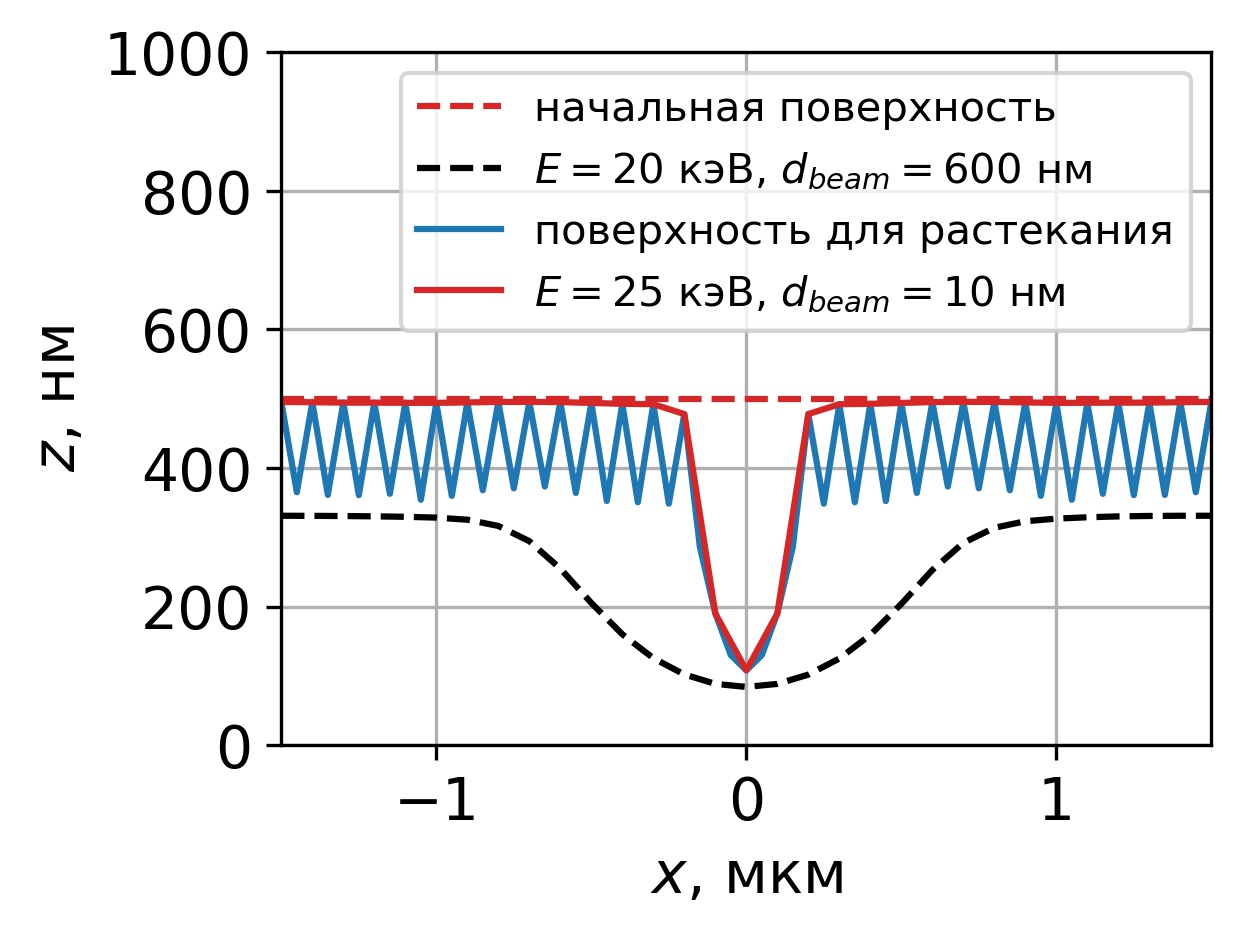
\includegraphics[width=\linewidth]{DEBER_resolution/resolution_25_um_300dpi} \\
		\vspace{-28.7ex} \\ \text{\hspace{0em} a}) \\ \vspace{28.7ex}
	\end{minipage}
	\begin{minipage}{0.48\textwidth}
		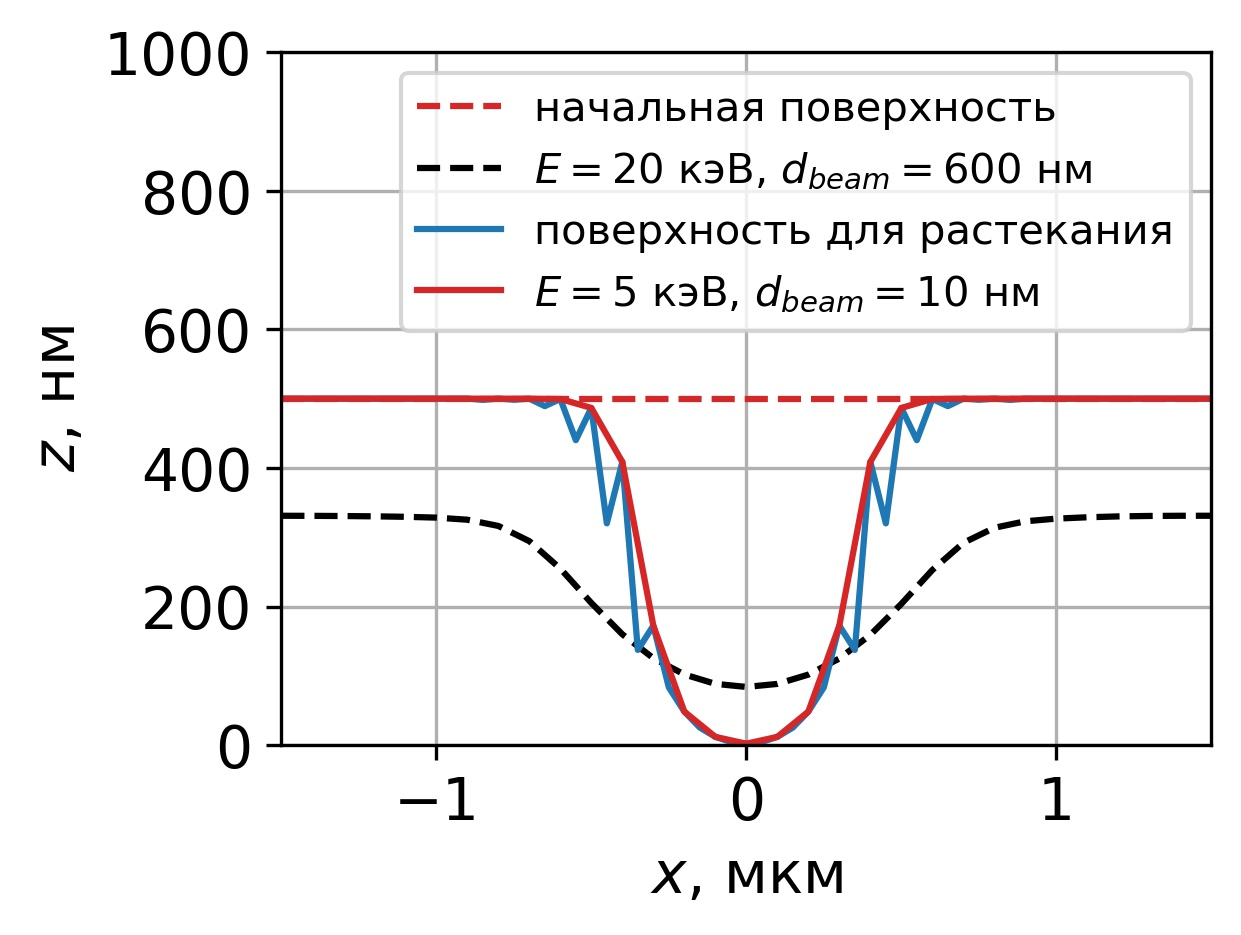
\includegraphics[width=\linewidth]{DEBER_resolution/resolution_5_um_300dpi} \\
		\vspace{-28.7ex} \\ \text{\hspace{-0.1em} б}) \\ \vspace{28.7ex}
	\end{minipage}
	\vspace{-3.5em}
	\caption{Линии, полученные методом СЭЛТР с максимальным разрешением с использованием узкого высокоэнергетического (25 кэВ, а)) или низкоэнергетического (5 кэВ, б)) пучка. Диаметр пучка составляет равным 10 нм, температура образцов -- 150 $^\circ$C/с, начальная толщина слоя ПММА -- 500 нм. Ток экспонирования равен 4.56 нА, скорость охлаждения образцов -- 10 $^\circ$C/с.}
	\label{fig:DEBER_resolution}
\end{figure}

Исходя из результатов моделирования, можно заключить, что использование узкого высокоэнергетического пучка способно повысить латеральное разрешение до величины около 300 нм. При этом также было установлено, что минимальная толщина слоя резиста в центре линии ограничена значением около 100 нм за, причиной чего является относительно большая средняя длина свободного пробега электронов при высоких энергиях, а также быстрое заполнение линии близлежащим резистом за счет процессов растекания. Использование узкого низкоэнергетического пучка, в свою очередь, обеспечивает латеральное разрешение около 600 нм, однако, делает возможным полное травление резиста в центре линии за счет относительно небольшой средней длины свободного пробега электронов при низких энергиях. При этом в обоих вышеописанных случаях угол наклона профиля на полувысоте составляет 65--72$^\circ$, что практически в три раза превышает угол наклона на полувысоте в экспериментальных структурах (24--27$^\circ$).

На основании результатов моделирования можно заключить, что при выборе оптимальных параметров экспонирования метод СЭЛТР позволяет получает практически идеальный синусоидальный профиль в резисте с периодом до половины микрометра, что соответствует 2000 штрихов на 1 мм. Как показано, на рис.~\ref{fig:DEBER_holo_2um}, синусоидальным профиль может быть достигнут как при полном или частичном наличии микрополостей в слое резиста (рис.~\ref{fig:DEBER_holo_2um} a), б)), так и при их отсутствии (рис.~\ref{fig:DEBER_holo_2um} в) и г)). Высота синусоидального профиля, получаемого методом СЭЛТР может варьироваться от 0 до 1500--200 нм в зависимости концентрации микрополостей в слое резисте.

Полученный в ПММА синусоидальный профиль может быть в дальнейшем покрыт металлом или перенесен в металл путем травления в реакторе индуктивно-связанной плазмы~\cite{Bruk_2016_mee}, что обеспечит получение отражательной синусоидальной дифракционной решетки. Таким образом, метод СЭЛТР может быть применен для получения синусоидальных дифракционных решеток с числом штрихов до 2000 1/мм, и отношением $d / \lambda$ в диапазоне 0--0.3, что обеспечит высокую эффективность решеток и широкий рабочий диапазон.

% 2 um
\begin{figure}[t!]
	\begin{minipage}{0.48\textwidth}
		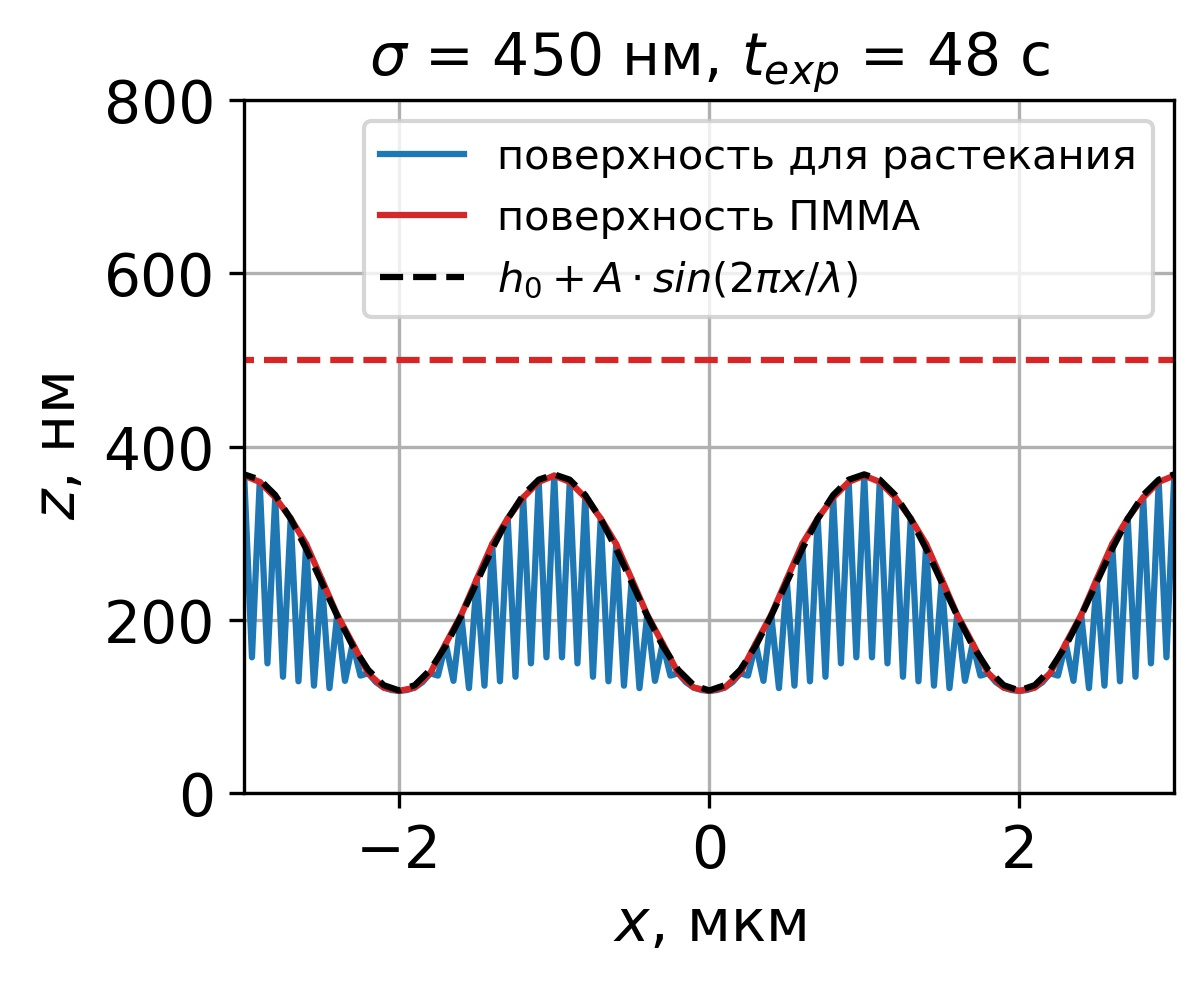
\includegraphics[width=0.9\linewidth]{DEBER_holo/2_um/holo_1C_s450_48s_um_300dpi} \\
		\vspace{-13em} \\ \text{\hspace{0em} a}) \\ \vspace{13em}
	\end{minipage}
	\begin{minipage}{0.48\textwidth}
		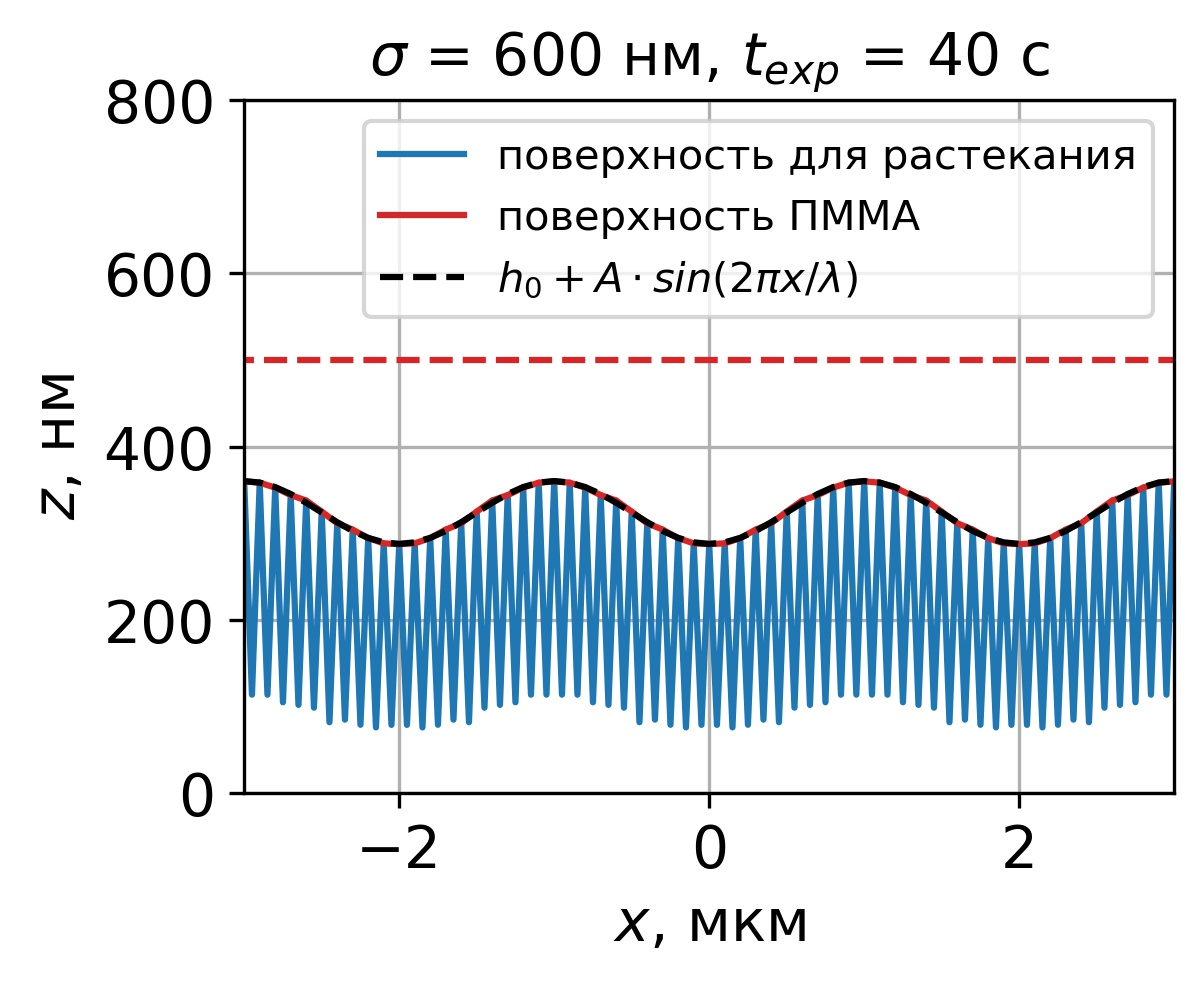
\includegraphics[width=0.9\linewidth]{DEBER_holo/2_um/holo_1C_s600_40s_um_300dpi} \\
		\vspace{-13em} \\ \text{\hspace{-0.1em} б}) \\ \vspace{13em}
	\end{minipage}
	
	\vspace{-3.5em}
	
	\begin{minipage}{0.48\textwidth}
		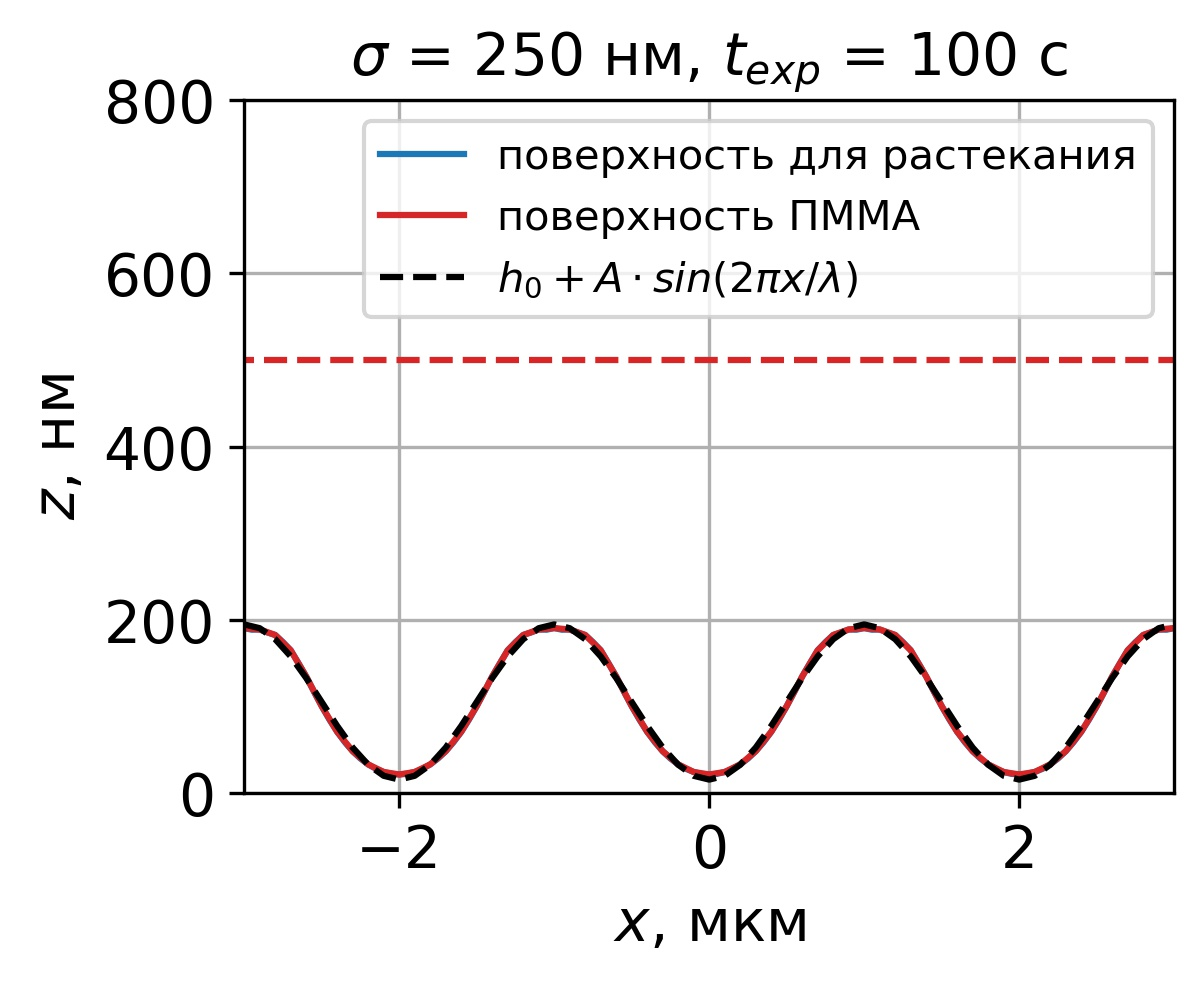
\includegraphics[width=0.9\linewidth]{DEBER_holo/2_um//holo_10C_s250_100s_um_300dpi} \\
		\vspace{-13em} \\ \text{\hspace{0em} в}) \\ \vspace{13em}
	\end{minipage}
	\begin{minipage}{0.48\textwidth}
		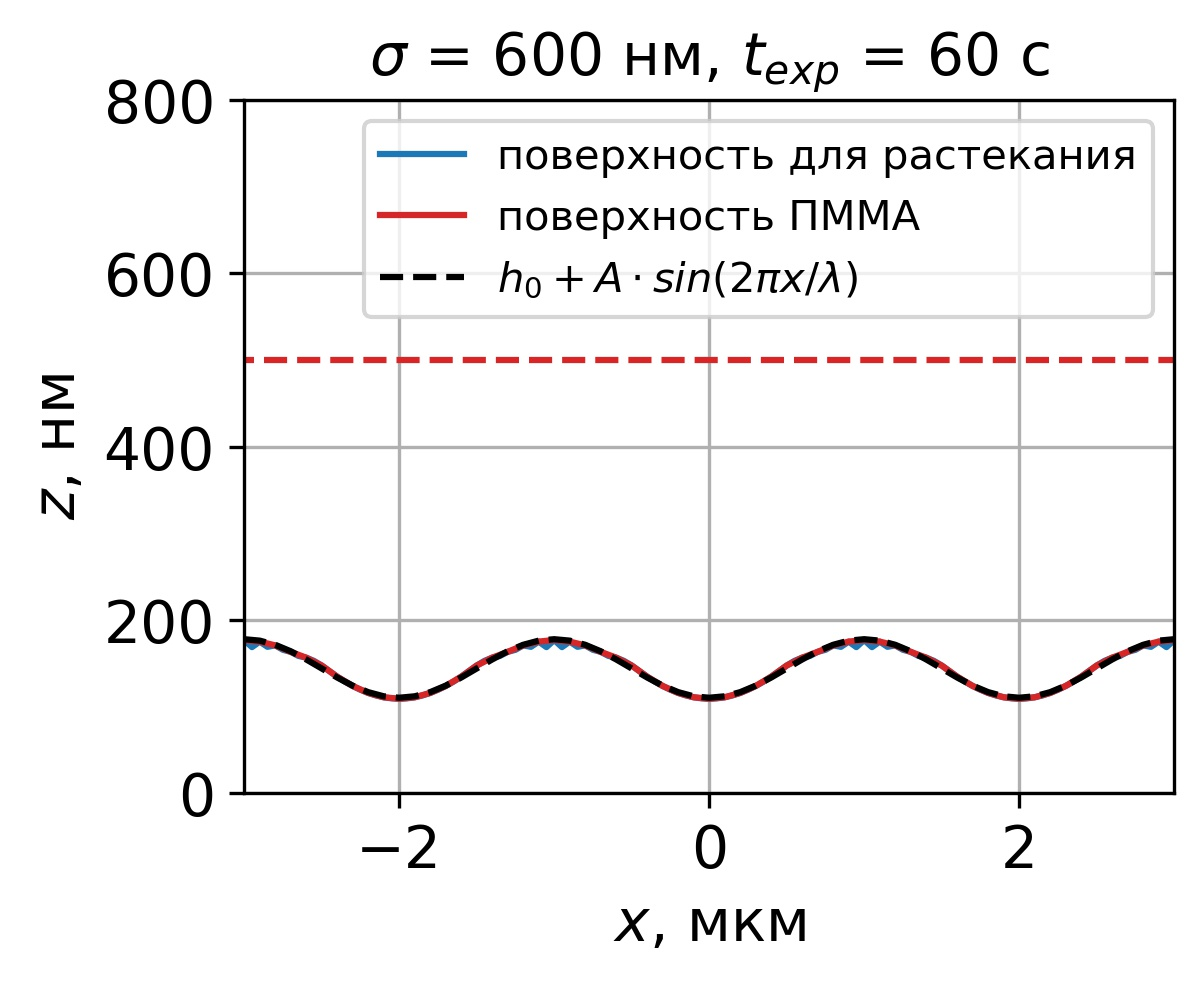
\includegraphics[width=0.9\linewidth]{DEBER_holo/2_um/holo_1C_s600_60s_um_300dpi} \\
		\vspace{-13em} \\ \text{\hspace{-0.1em} г}) \\ \vspace{13em}
	\end{minipage}
	\vspace{-3em}
	\caption{Промоделированные синусоидальные профили с периодом 2~мкм, полученные в слое ПММА с начальной толщиной 500 нм. Температура образца составляла $T$ = 150 $^\circ$C, ток в пучке -- 4.56 нА, распределение плотности тока в пучке считается нормальным со среднеквадратичным отношением $\sigma$. Значения $\sigma$ и $t_{exp}$ подбираются для получения синусоидального профиля. После экспонирования образец а) охлаждался со скоростью 10 $^\circ$C/с, образцы б)--г) -- со скоростью 1 $^\circ$C/с. 
		%		Черная пунктирная линия обозначает подгонку промоделированного профиля функцией синус.
	}
	\label{fig:DEBER_holo_2um}
\end{figure}


Разработанный алгоритм моделирования линии, получаемой в процессе СЭЛТР, вообще говоря, может быть использован для определения результирующего профиля при произвольном экспонировании по области на поверхности резиста. В качестве демонстрации возможностей алгоритма были промоделированы профили, получаемые при экспонировании электронным лучом, плотность тока в котором описывалась суммой двух (рис.~\ref{fig:DEBER_multibeam} a)) или четырех ((рис.~\ref{fig:DEBER_multibeam} б)) функций Гаусса со среднеквадратичным отклонением 200 нм. 

\begin{figure}[h]
	\begin{minipage}{0.48\textwidth}
		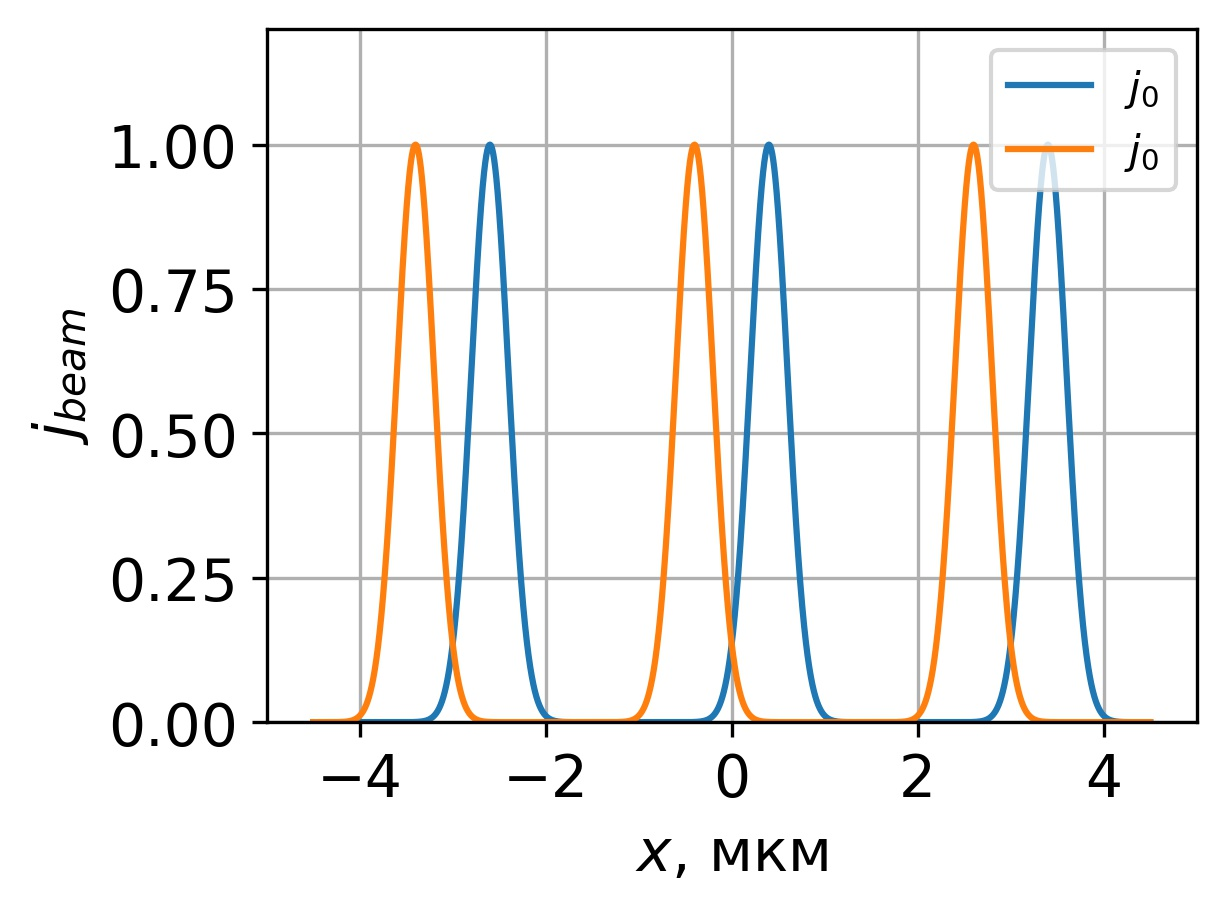
\includegraphics[width=0.9\linewidth]{DEBER_asymmetric/pm_400_colors} \\
		\vspace{-13em} \\ \text{\hspace{0em} a}) \\ \vspace{13em}
	\end{minipage}
	\begin{minipage}{0.48\textwidth}
		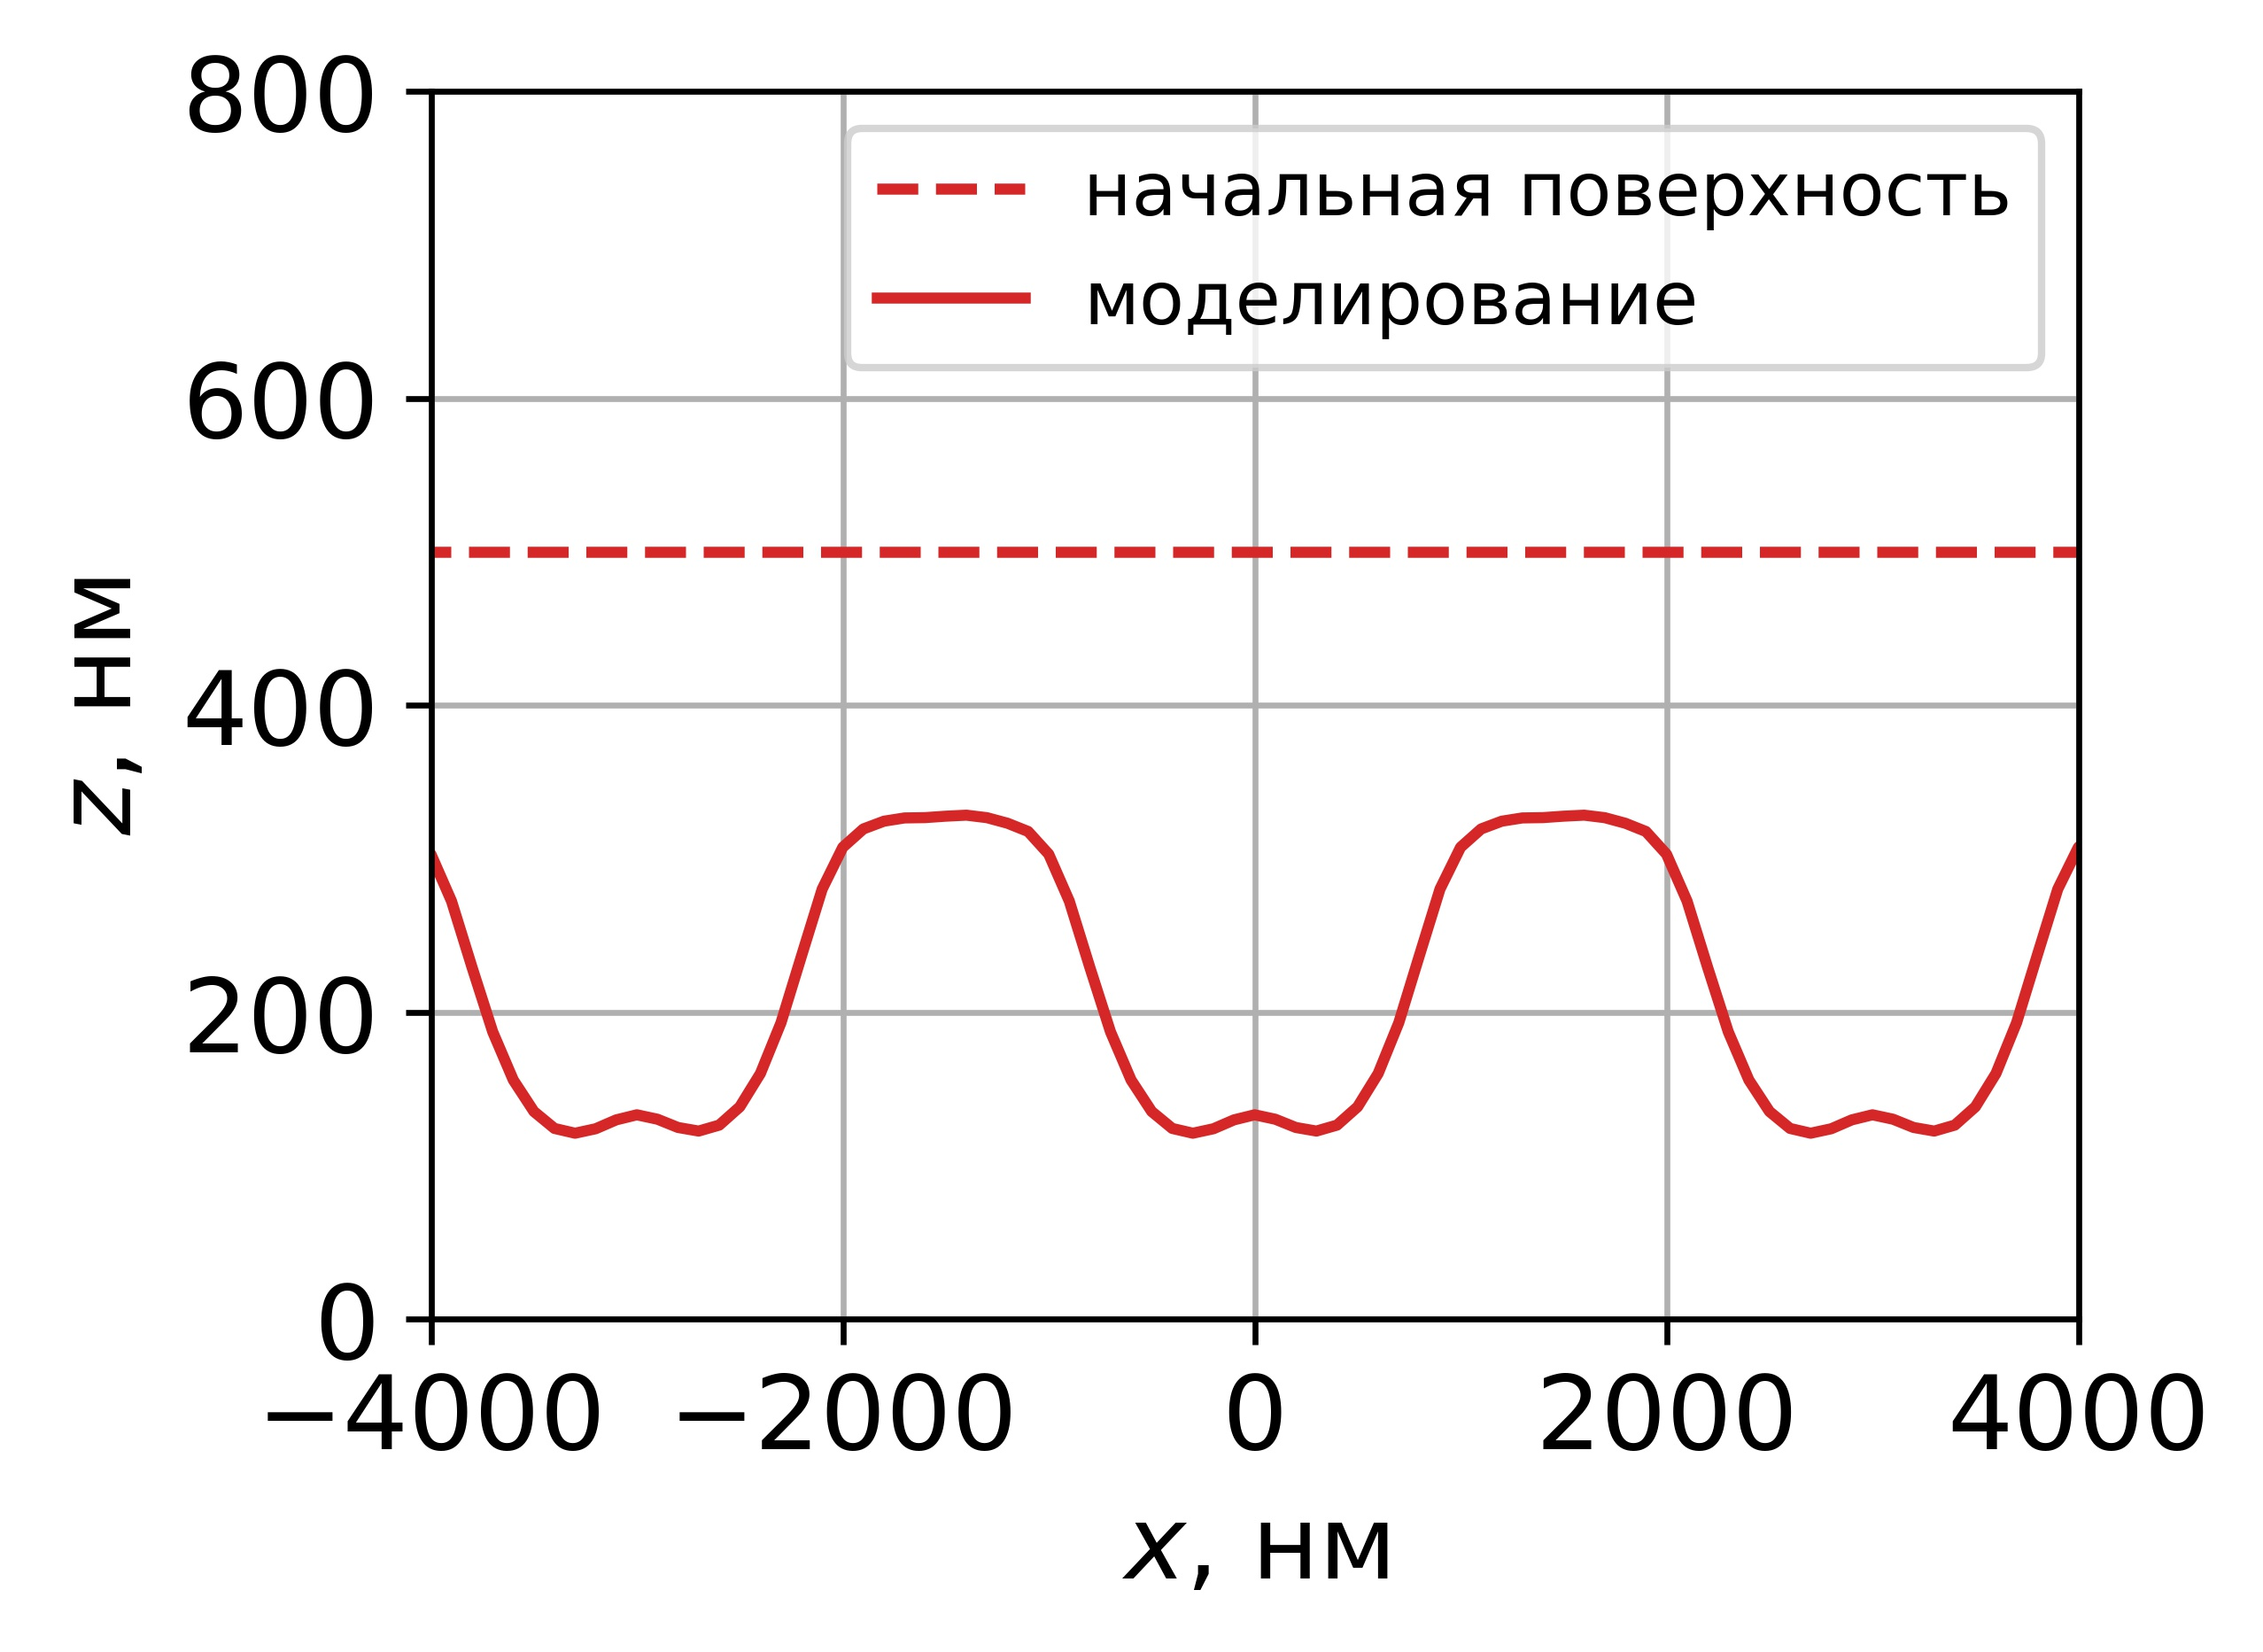
\includegraphics[width=0.9\linewidth]{DEBER_asymmetric/2beams_profile} \\
		\vspace{-13em} \\ \text{\hspace{-0.1em} б}) \\ \vspace{13em}
	\end{minipage}
	
	\vspace{-3em}
	
	\begin{minipage}{0.48\textwidth}
		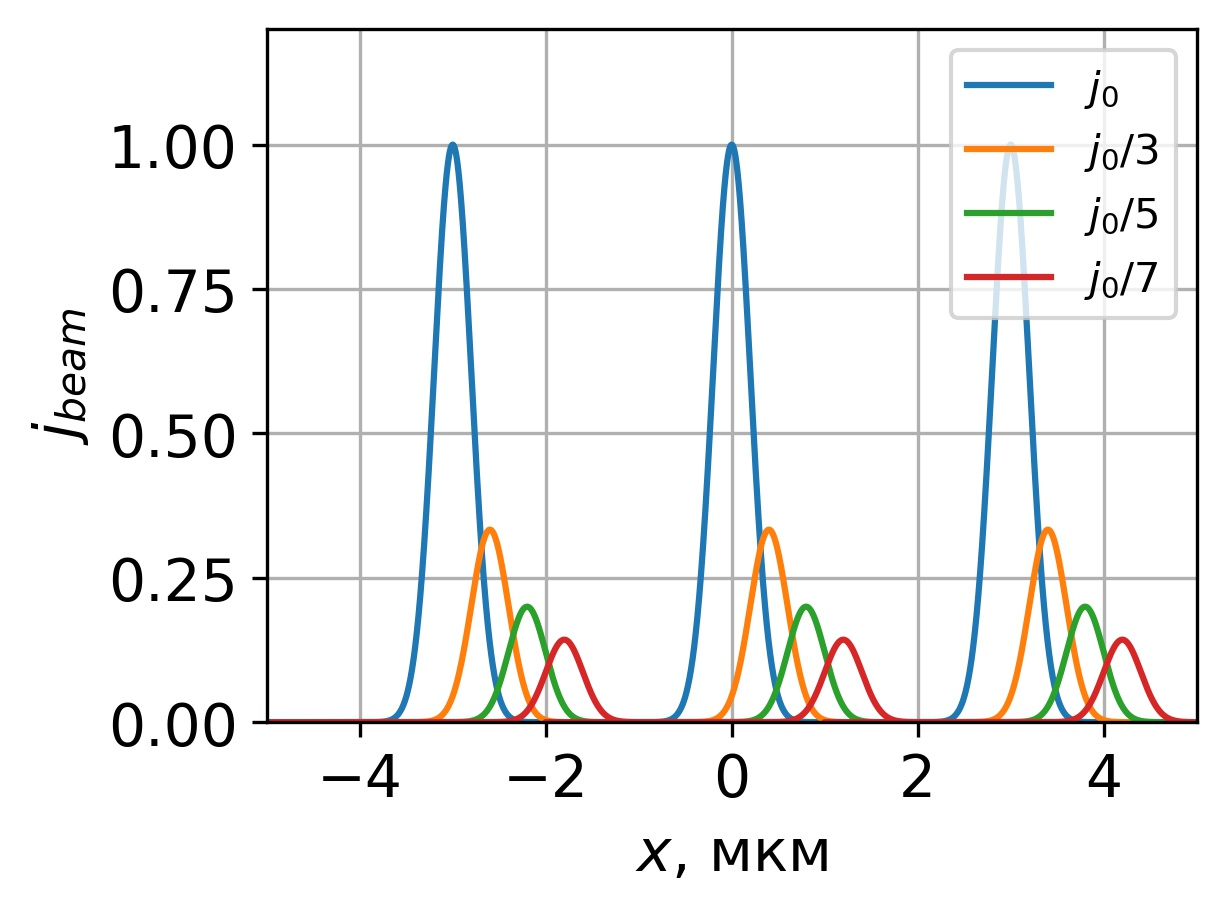
\includegraphics[width=0.9\linewidth]{DEBER_asymmetric/asymmetric} \\
		\vspace{-13em} \\ \text{\hspace{0em} в}) \\ \vspace{13em}
	\end{minipage}
	\begin{minipage}{0.48\textwidth}
		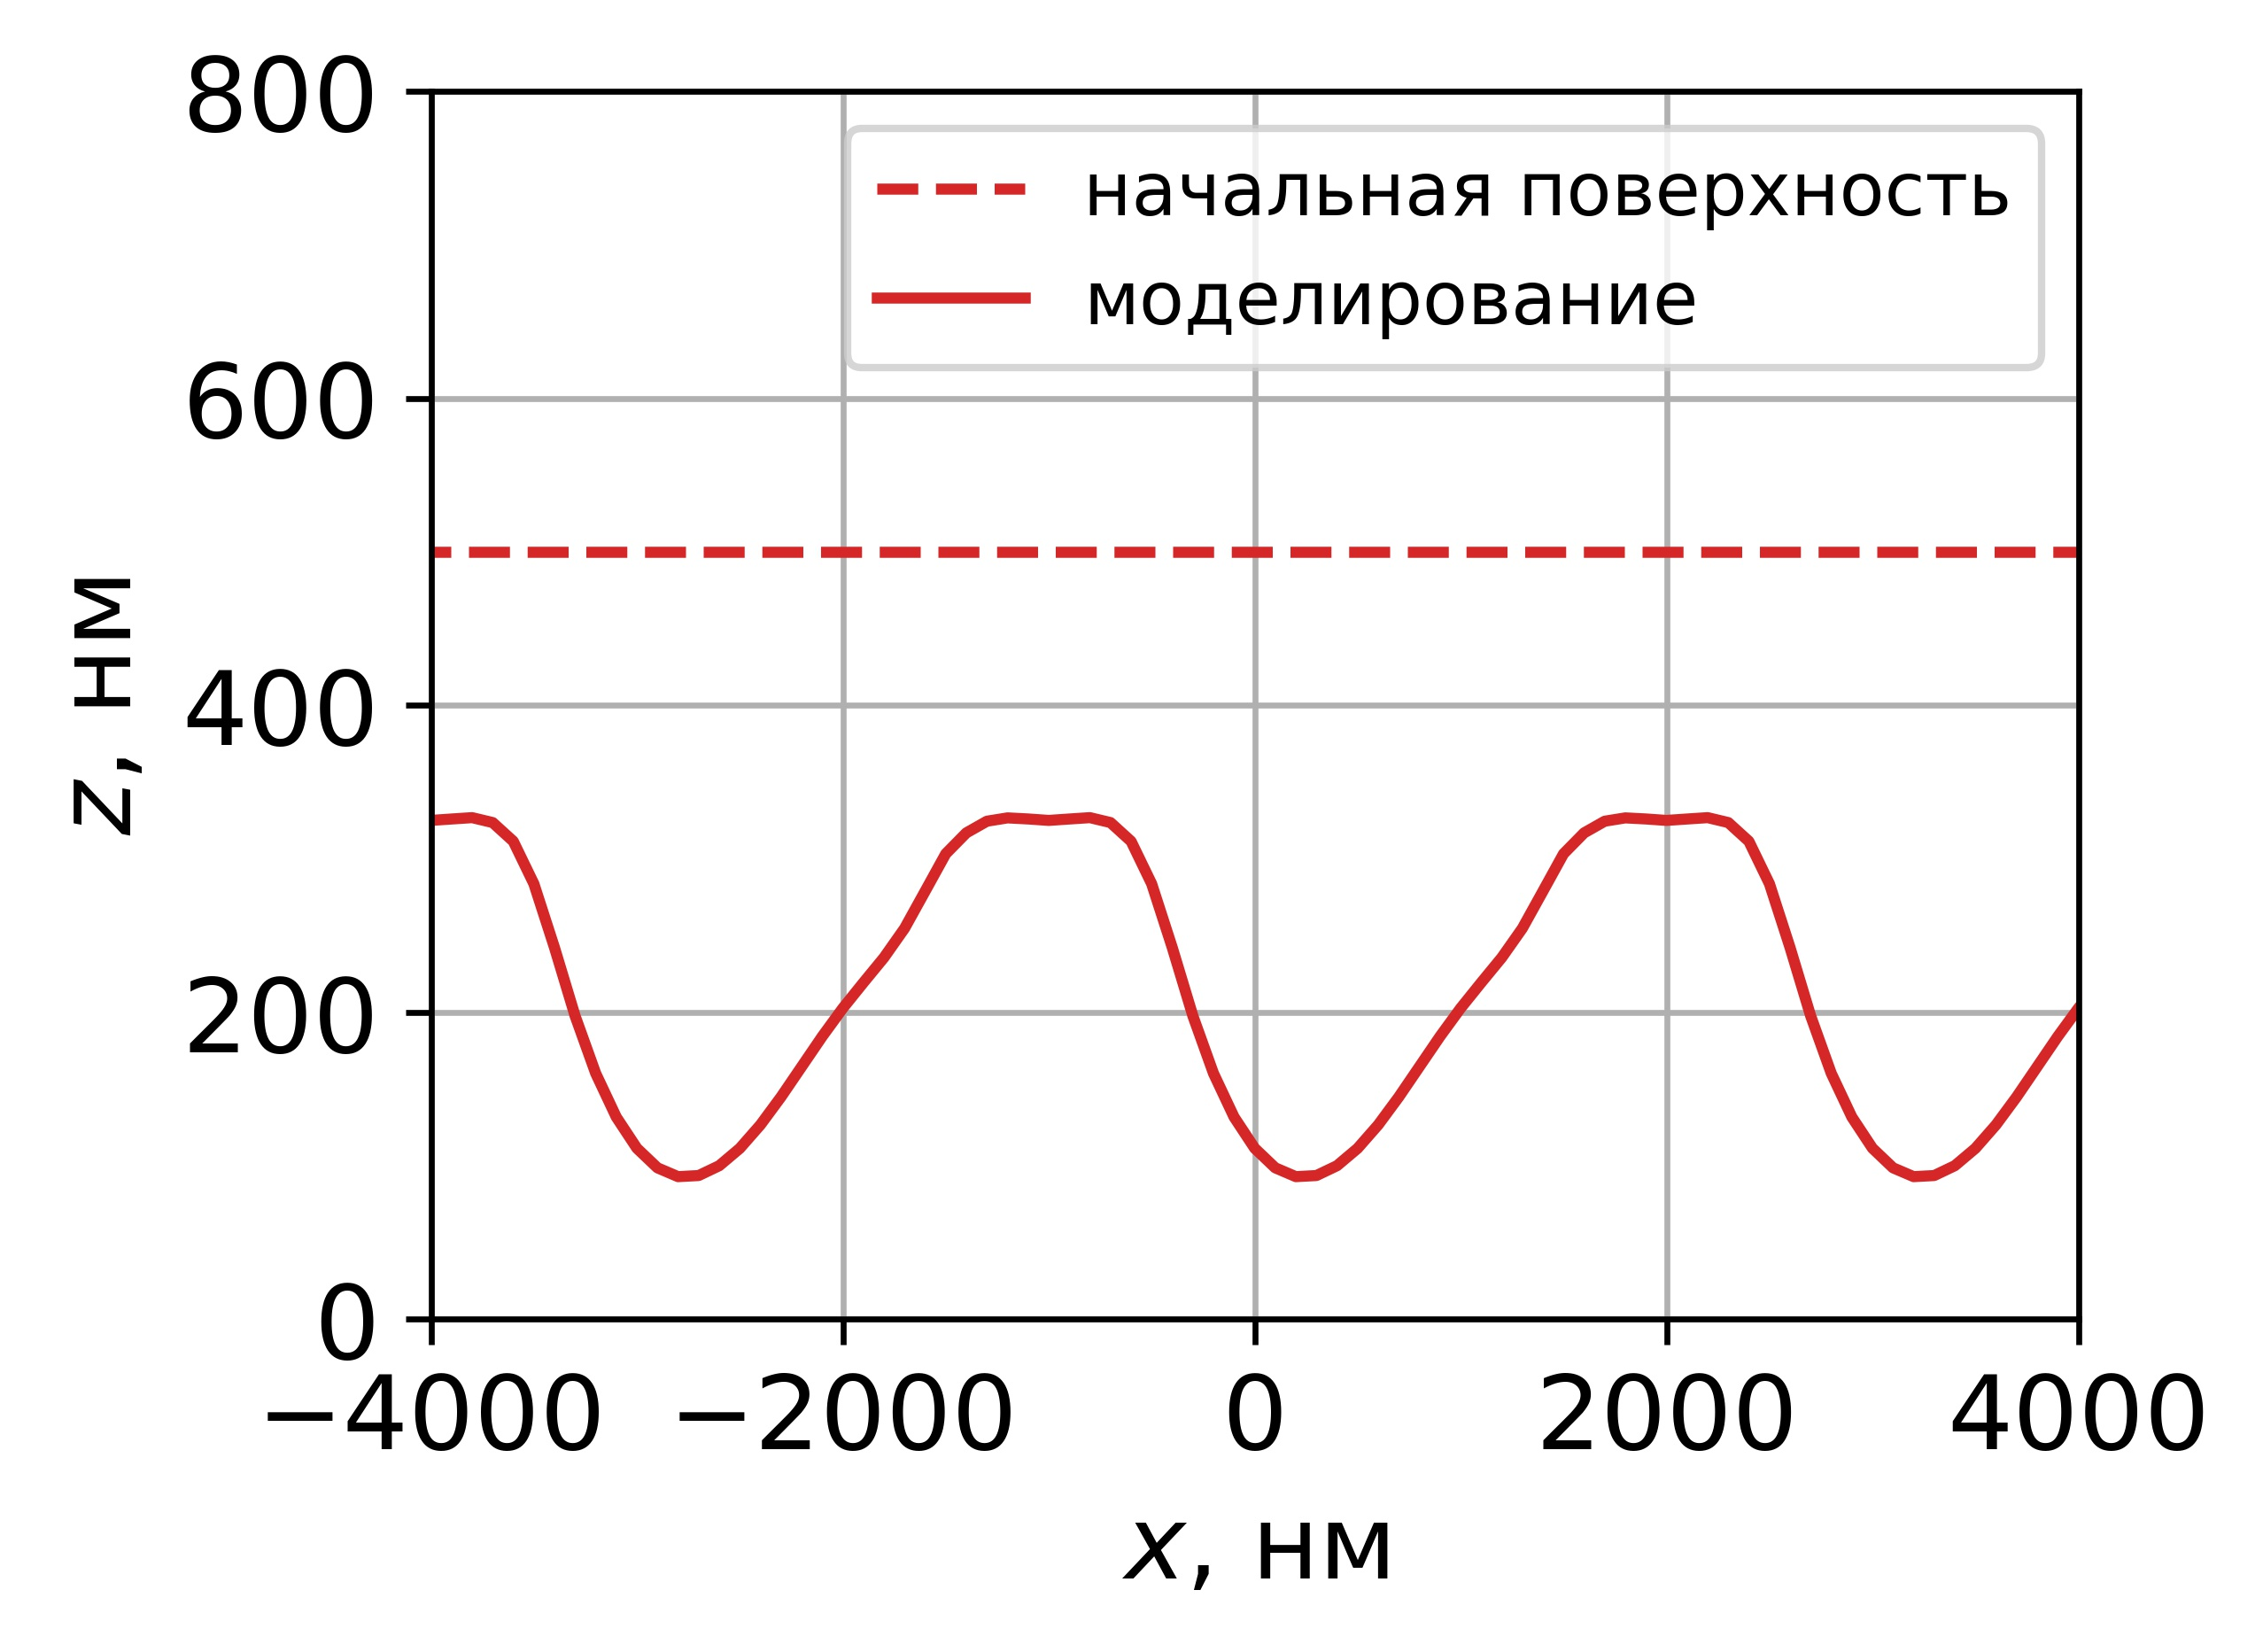
\includegraphics[width=0.9\linewidth]{DEBER_asymmetric/4beams_profile} \\
		\vspace{-13em} \\ \text{\hspace{-0.1em} г}) \\ \vspace{13em}
	\end{minipage}
	\vspace{-3em}
	\caption{Промоделированные периодические профили с периодом 3 мкм, полученные в слое ПММА с начальной толщиной 500 нм методом СЭЛТР при экспонировании по области с различным распределением плотности тока в пучке. Температура образца при экспонировании -- 150 $^\circ$C/с, время экспонирования -- 100 с, доза экспонирования -- 3 нКл/см (доза относится к единице длины линии, экспонируемой двумя пучками в случае a) и четырьмя пучками в случае в)). Охлаждение проводилось в соответствии с экспериментальной кривой охлаждения.}
	\label{fig:DEBER_multibeam}
\end{figure}
